\chapter{Sysvinit 项目工具简介}

\section{项目背景介绍}

init 进程是 Unix 和 Linux 系统中,用来产生其他所有进程的程序。init
的进程号 pid 是1,它是其他所有进程的祖先。 关于 init
进程的实现方法,历史上有过两种实现方案,BSD 风格和 SysV 风格。

BSD 风格比较简单,也就是通常在很多嵌入式Linux系统中经常可以看到的 /etc/rc
脚本方式,init
进程负责从这个启动脚本中读取一系列需要执行的程序,依次执行直到最后启动
getty (基于文本模式的终端)或者 X (基于图形界面的窗口系统)。

Sysv 相对复杂一些,它提出了一个关于 runlevel
运行级别的概念,为了实现启动系统到不同的运行级别,它引入了一个
/etc/inittab 的启动配置文件,通过这个配置文件指定的 initdefault
的值(从0-6或者S),可以引导系统分别进入到单用户模式,多用户模式(还可以分为有网络连接和无网络连接两种),多用户带图形界面方式
和用户自定义方式等,同时也可以引导系统到关机模式和重启模式。

大部分 Linux 的发行版都是采用和 System V init 相兼容的方式启动,为了配置
init 进程的这些运行级别和功能,sysvinit 的作者 Miquel van Smoorenburg
开发实现了一组软件包来完成这些功能。这个软件包就是我们所要研究的
sysvinit
项目,其中所包含的工具在下面我们要介绍的项目技术架构中会详细阐述。

下面我们列举一些有关 sysvinit 项目所需要用到的资源,以便了解和查看。

\subsection{项目相关资源链接}

\begin{itemize}
\item
  项目主页\\\url{https://savannah.nongnu.org/projects/sysvinit/}
\item
  源码下载\\\url{http://download.savannah.gnu.org/releases/sysvinit/}
\item
  开发成员
  \begin{itemize}
  \item
    Petter Reinholdtsen
  \item
    Roger Leigh
  \item
    Dr.~Werner Fink
  \end{itemize}
\end{itemize}
\subsection{其他类似软件包}

事实上,从 sysvinit
产生之后,又出现了许多类似的项目,其主要功能都是来帮助内核最终完成启动用户应用程序。我们列举其中一些比较常见知名的项目,作为后继研究的参考。

\begin{itemize}
\item
  Upstart\\最早在 Ubuntu 6.10 中广泛采用的,基于事件机制 event-based
  的,异步方式工作的 init 进程方案,完全可以兼容 sysvinit 的脚本。
  现在也被很多其他操作系统发行版所采用,例如 Google Chrome OS,HP Web
  OS,中均采用了 upstart 来作为默认的init启动程序。
\item
  SystemStarter\\在 Mac OS X v10.4 之前所采用的 BSD 风格的 init
  进程方案。
\item
  launchd\\在 Mac OS X v10.4 和之后所采用,它会启动 SystemStarter 来处理
  rc.local 脚本。
\item
  systemd\\能够提供更好的服务依赖性的支持,允许系统启动期间能够并发完成更多工作,减小shell的开销。
  systemd 在 Fedora 15 和 openSUSE 12.1 中所采用。
\end{itemize}
\section{项目技术架构}

Sysvinit
软件包是一组Linux工具集,包含控制启动,运行和关闭所有其他程序的工具。

具体包含有如下这些命令:

\begin{itemize}
\item
  init
\item
  telinit (链接到 init)
\item
  sulogin
\item
  halt
\item
  poweroff (链接到 halt)
\item
  reboot (链接到 halt)
\item
  shutdown
\item
  last, lastb (链接到 last)
\item
  killall5
\item
  pidof (链接到 killall5)
\item
  mesg
\item
  wall
\item
  runlevel
\item
  utmpdump
\end{itemize}
这些命令多达13条,我们可以把它们按功能和用途进行归类。

\subsection{核心命令 init/telinit}

init 是所有命令中的核心,也是该项目最重要的输出成果,提供一个可以和 Kernel
进行对接的 init 程序,实现支持不同运行级别的启动方式。 telinit 是一个
init 程序的软链接,用来通知 init 进程切换运行级别。

\subsection{关机命令 halt/shutdown/poweroff/reboot}

这4条命令都是和系统关机有关,名字很接近。其中 shutdown
命令是这里面的核心命令,halt 命令是通过调用 shutdown 命令来完成功能的。
poweroff 和 reboot 这2条命令,都是指向 halt
命令的软链接。我们把它们可以统称为关机命令。

\subsection{运行级别命令 sulogin/runlevel}

sulogin 是为单用户运行级别提供的登录验证程序,用户运行这个命令就会以 root
方式进入单用户模式。 runlevel
是一条测试命令,检查当前的运行级别,和之前上一个运行级别,打印出来给用户以便了解。

\subsection{进程/消息相关命令 mesg/wall/killall5/pidof}

这里面的命令都是和进程/消息有关的。mesg 是给某个用户和终端发消息,wall
是给全部登录用户发消息。 killall5 是向所有进程发送 SIGKILL
消息,杀死进程。 pidof 是一个 killall5 的软链接,打印出对应输入进程名
progname 的进程号 pid。

\subsection{日志相关命令 bootlogd/utmpdump}

bootlogd 命令可以设置启动时候输出的信息到日志文件中,默认的日志文件是
/var/log/boot 。 utmpdump 命令可以实现以便于查看的格式输出 /var/run/utmp
文件日志内容。

\subsection{文件系统相关命令 mountpoint/fstab-decode}

mountpoint 命令用来检查某个目录是否是一个挂载点,也就是 mount
上来的目录。例如 / 和 /proc 一般都是,但 /etc /lib 一般不是。
fstab-decode 命令用来运行一条命令,在这个命令中可以加上一些参数,由
fstab-decode 来解析。

\begin{figure}[htbp]
\centering
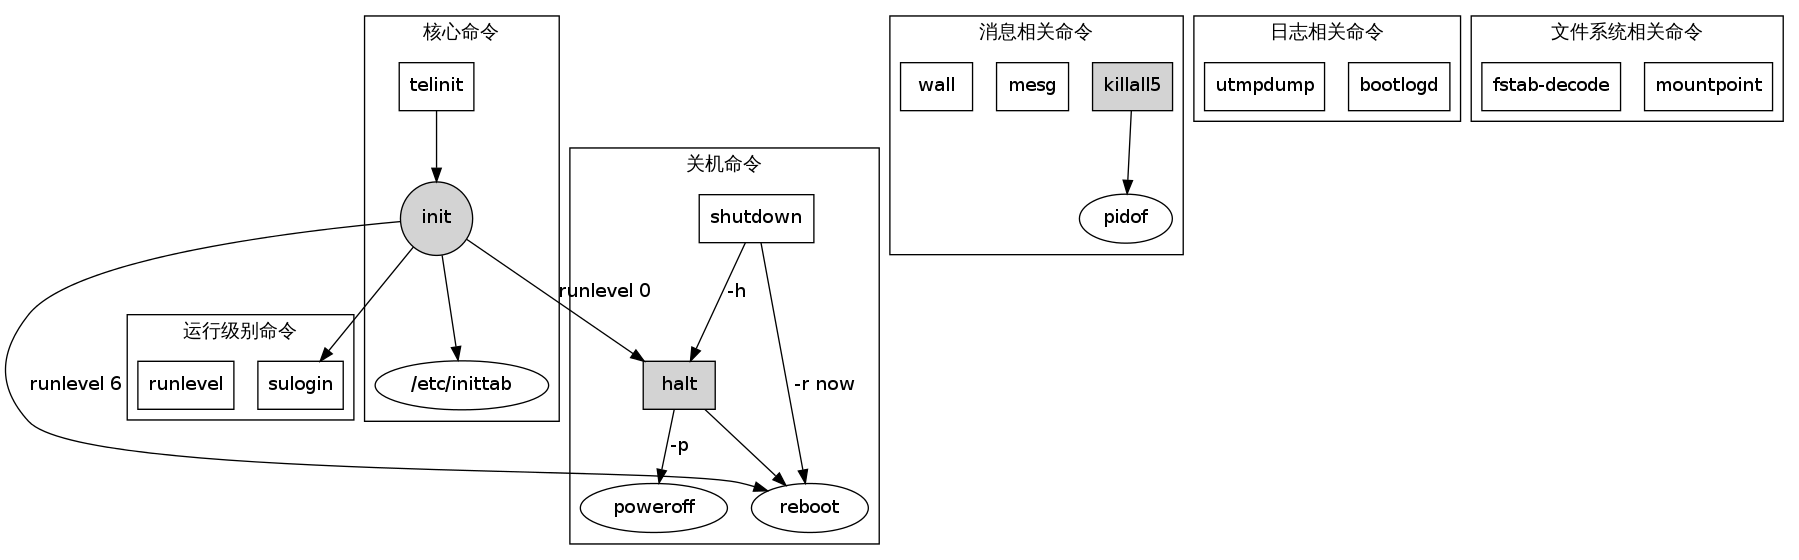
\includegraphics{./figures/sys.png}
\caption{sysvinit 系统层次结构图}
\end{figure}

\chapter{Sysvinit 项目概要分析}

\section{代码实现概要分析}

我们目前所要分析的源码压缩包为 2.88 版本的,这个版本的发布时间是
26-Mar-2010。

\subsection{源码目录结构}

{\begin{shaded}\begin{verbatim}
$ tree
.
├── contrib
│   ├── alexander.viro
│   ├── notify-pam-dead.patch
│   ├── start-stop-daemon.c
│   ├── start-stop-daemon.README
│   ├── TODO
│   └── zefram-patches
├── COPYING
├── COPYRIGHT
├── doc
│   ├── bootlogd.README
│   ├── Changelog
│   ├── Install
│   ├── Propaganda
│   └── sysvinit-2.86.lsm
├── Makefile
├── man
│   ├── bootlogd.8
│   ├── bootlogd.8.todo
│   ├── fstab-decode.8
│   ├── halt.8
│   ├── init.8
│   ├── initscript.5
│   ├── inittab.5
│   ├── killall5.8
│   ├── last.1
│   ├── lastb.1
│   ├── mesg.1
│   ├── mountpoint.1
│   ├── pidof.8
│   ├── poweroff.8
│   ├── reboot.8
│   ├── runlevel.8
│   ├── shutdown.8
│   ├── sulogin.8
│   ├── telinit.8
│   ├── utmpdump.1
│   └── wall.1
├── obsolete
│   ├── bootlogd.init
│   ├── powerd.8
│   ├── powerd.c
│   ├── powerd.cfg
│   ├── powerd.README
│   ├── README.RIGHT.NOW
│   └── utmpdump.c.OLD
├── README
└── src
    ├── a.out
    ├── bootlogd.c
    ├── dowall.c
    ├── fstab-decode.c
    ├── halt.c
    ├── hddown.c
    ├── ifdown.c
    ├── init.c
    ├── init.h
    ├── initreq.h
    ├── initscript.sample
    ├── killall5.c
    ├── last.c
    ├── Makefile
    ├── mesg.c
    ├── mountpoint.c
    ├── oldutmp.h
    ├── paths.h
    ├── reboot.h
    ├── runlevel.c
    ├── set.h
    ├── shutdown.c
    ├── sulogin.c
    ├── utmp.c
    ├── utmpdump.c
    └── wall.c

5 directories, 69 files
\end{verbatim}\end{shaded}}
\subsection{源文件代码量分析}

src 目录下的源码文件共 17 个,全部代码量一共 9350 行,接近一万行。其中
init.c 是这里面代码量最大的,约有3000行。killall5.c
约有1100行。其他的源代码都在1000行以内。

{\begin{shaded}\begin{verbatim}
$ ls *.c -l | wc -l
17
$ ls *.c -l | awk '{print $9}' | xargs wc -l | sort -n
    53 runlevel.c
    86 fstab-decode.c
   109 ifdown.c
   122 wall.c
   124 mesg.c
   128 mountpoint.c
   253 dowall.c
   264 utmp.c
   302 utmpdump.c
   315 halt.c
   568 hddown.c
   607 sulogin.c
   690 bootlogd.c
   762 shutdown.c
   928 last.c
  1104 killall5.c
  2935 init.c
  9350 total
\end{verbatim}\end{shaded}}
\subsection{Makefile 分析}

{\begin{shaded}\begin{verbatim}
 93 init:           LDLIBS += $(INITLIBS) $(STATIC)
 94 init:           init.o init_utmp.o
 95 
 96 halt:           halt.o ifdown.o hddown.o utmp.o reboot.h
 97 
 98 last:           last.o oldutmp.h
 99 
100 mesg:           mesg.o
101 
102 mountpoint:     mountpoint.o
103 
104 utmpdump:       utmpdump.o
105 
106 runlevel:       runlevel.o
107 
108 sulogin:        LDLIBS += $(SULOGINLIBS) $(STATIC)
109 sulogin:        sulogin.o
110 
111 wall:           dowall.o wall.o
112 
113 shutdown:       dowall.o shutdown.o utmp.o reboot.h
114 
115 bootlogd:       LDLIBS += -lutil
116 bootlogd:       bootlogd.o
\end{verbatim}\end{shaded}}
以上是生成可执行文件的 Makefile
关键片段。从这里可以大致看出,每个可执行文件的生成,需要依赖于哪些目标文件,也就是由哪些源码文件生成的。例如
init 程序,是由 init.c init\_utmp.c 这2个文件生成,如果我们要研究 init
程序的源码,就需要读懂这2个源码文件。

\section{项目下载编译执行}

\subsection{wget下载源码包}

\begin{figure}[htbp]
\centering
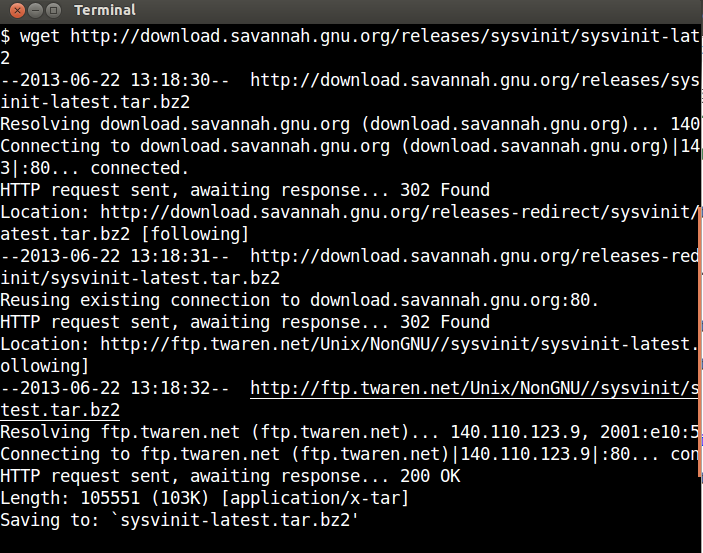
\includegraphics{./pictures/1-1-wget.png}
\caption{wget下载源码包}
\end{figure}

{\begin{shaded}\begin{verbatim}
$ wget http://download.savannah.gnu.org/releases/sysvinit/sysvinit-latest.tar.bz2
--2013-06-22 13:18:30--  http://download.savannah.gnu.org/releases/sysvinit/sysvinit-latest.tar.bz2
Resolving download.savannah.gnu.org (download.savannah.gnu.org)... 140.186.70.73
Connecting to download.savannah.gnu.org (download.savannah.gnu.org)|140.186.70.73|:80... connected.
HTTP request sent, awaiting response... 302 Found
Location: http://download.savannah.gnu.org/releases-redirect/sysvinit/sysvinit-latest.tar.bz2 [following]
--2013-06-22 13:18:31--  http://download.savannah.gnu.org/releases-redirect/sysvinit/sysvinit-latest.tar.bz2
Reusing existing connection to download.savannah.gnu.org:80.
HTTP request sent, awaiting response... 302 Found
Location: http://ftp.twaren.net/Unix/NonGNU//sysvinit/sysvinit-latest.tar.bz2 [following]
--2013-06-22 13:18:32--  http://ftp.twaren.net/Unix/NonGNU//sysvinit/sysvinit-latest.tar.bz2
Resolving ftp.twaren.net (ftp.twaren.net)... 140.110.123.9, 2001:e10:5c00:5::9
Connecting to ftp.twaren.net (ftp.twaren.net)|140.110.123.9|:80... connected.
HTTP request sent, awaiting response... 200 OK
Length: 105551 (103K) [application/x-tar]
Saving to: `sysvinit-latest.tar.bz2'

100%[======================================>] 105,551     45.1K/s   in 2.3s    

2013-06-22 13:18:35 (45.1 KB/s) - `sysvinit-latest.tar.bz2' saved [105551/105551]
\end{verbatim}\end{shaded}}
\subsection{tar解压源码包}

\begin{figure}[htbp]
\centering
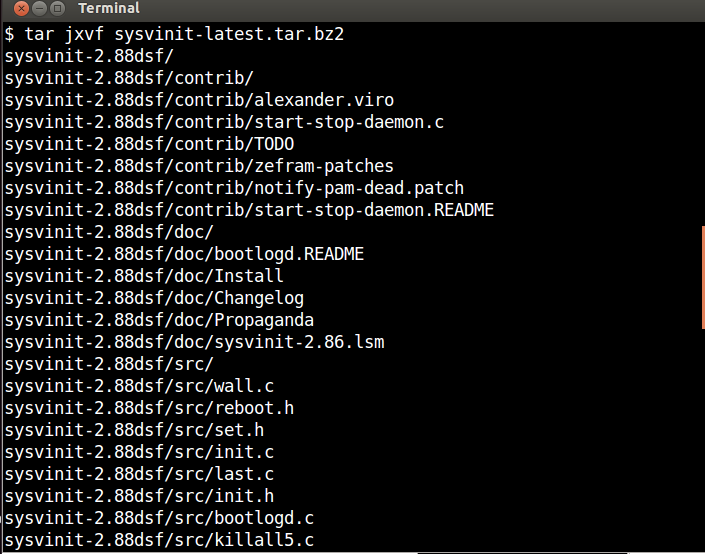
\includegraphics{./pictures/1-2-tar.png}
\caption{tar解压源码包}
\end{figure}

{\begin{shaded}\begin{verbatim}
$ tar jxvf sysvinit-latest.tar.bz2 
sysvinit-2.88dsf/
sysvinit-2.88dsf/contrib/
sysvinit-2.88dsf/contrib/alexander.viro
sysvinit-2.88dsf/contrib/start-stop-daemon.c
sysvinit-2.88dsf/contrib/TODO
sysvinit-2.88dsf/contrib/zefram-patches
sysvinit-2.88dsf/contrib/notify-pam-dead.patch
sysvinit-2.88dsf/contrib/start-stop-daemon.README
sysvinit-2.88dsf/doc/
sysvinit-2.88dsf/doc/bootlogd.README
sysvinit-2.88dsf/doc/Install
sysvinit-2.88dsf/doc/Changelog
sysvinit-2.88dsf/doc/Propaganda
sysvinit-2.88dsf/doc/sysvinit-2.86.lsm
sysvinit-2.88dsf/src/
sysvinit-2.88dsf/src/wall.c
sysvinit-2.88dsf/src/reboot.h
sysvinit-2.88dsf/src/set.h
sysvinit-2.88dsf/src/init.c
sysvinit-2.88dsf/src/last.c
sysvinit-2.88dsf/src/init.h
sysvinit-2.88dsf/src/bootlogd.c
sysvinit-2.88dsf/src/killall5.c
sysvinit-2.88dsf/src/utmpdump.c
sysvinit-2.88dsf/src/shutdown.c
sysvinit-2.88dsf/src/mountpoint.c
sysvinit-2.88dsf/src/sulogin.c
sysvinit-2.88dsf/src/fstab-decode.c
sysvinit-2.88dsf/src/initreq.h
sysvinit-2.88dsf/src/dowall.c
sysvinit-2.88dsf/src/hddown.c
sysvinit-2.88dsf/src/paths.h
sysvinit-2.88dsf/src/utmp.c
sysvinit-2.88dsf/src/ifdown.c
sysvinit-2.88dsf/src/initscript.sample
sysvinit-2.88dsf/src/halt.c
sysvinit-2.88dsf/src/oldutmp.h
sysvinit-2.88dsf/src/mesg.c
sysvinit-2.88dsf/src/Makefile
sysvinit-2.88dsf/src/runlevel.c
sysvinit-2.88dsf/COPYING
sysvinit-2.88dsf/COPYRIGHT
sysvinit-2.88dsf/man/
sysvinit-2.88dsf/man/bootlogd.8
sysvinit-2.88dsf/man/killall5.8
sysvinit-2.88dsf/man/shutdown.8
sysvinit-2.88dsf/man/bootlogd.8.todo
sysvinit-2.88dsf/man/sulogin.8
sysvinit-2.88dsf/man/fstab-decode.8
sysvinit-2.88dsf/man/mesg.1
sysvinit-2.88dsf/man/initscript.5
sysvinit-2.88dsf/man/inittab.5
sysvinit-2.88dsf/man/poweroff.8
sysvinit-2.88dsf/man/wall.1
sysvinit-2.88dsf/man/halt.8
sysvinit-2.88dsf/man/reboot.8
sysvinit-2.88dsf/man/last.1
sysvinit-2.88dsf/man/runlevel.8
sysvinit-2.88dsf/man/lastb.1
sysvinit-2.88dsf/man/pidof.8
sysvinit-2.88dsf/man/init.8
sysvinit-2.88dsf/man/utmpdump.1
sysvinit-2.88dsf/man/mountpoint.1
sysvinit-2.88dsf/man/telinit.8
sysvinit-2.88dsf/obsolete/
sysvinit-2.88dsf/obsolete/powerd.c
sysvinit-2.88dsf/obsolete/powerd.8
sysvinit-2.88dsf/obsolete/utmpdump.c.OLD
sysvinit-2.88dsf/obsolete/README.RIGHT.NOW
sysvinit-2.88dsf/obsolete/bootlogd.init
sysvinit-2.88dsf/obsolete/powerd.README
sysvinit-2.88dsf/obsolete/powerd.cfg
sysvinit-2.88dsf/Makefile
sysvinit-2.88dsf/README
$ 

$ ls
Makefile  pdf  sysvinit-2.88dsf  sysvinit-latest.tar.bz2

$ ls sysvinit-2.88dsf/
contrib  COPYRIGHT  Makefile  obsolete  src
COPYING  doc        man       README
$ 
\end{verbatim}\end{shaded}}
\subsection{修改 Makefile}

增添11行的 CC=gcc,注释掉 13,14行有关 CFLAGS
的定义,否则编译会出很多的警告错误。

{\begin{shaded}\begin{verbatim}
$ vi Makefile 

10 
11 CC=gcc
12 CPPFLAGS =
13 #CFLAGS ?= -ansi -O2 -fomit-frame-pointer
14 #override CFLAGS += -W -Wall -D_GNU_SOURCE -DDEBUG
15 override CFLAGS += -D_GNU_SOURCE -DDEBUG
16 STATIC  =
17 
...
\end{verbatim}\end{shaded}}
在80行处添加83行处的赋值,增加链接时 -lcrypt 选项

{\begin{shaded}\begin{verbatim}
80 SULOGINLIBS     += -lcrypt
81 # Additional libs for GNU libc.
82 ifneq ($(wildcard /usr/lib*/libcrypt.a),)
83   SULOGINLIBS   += -lcrypt
84 endif
85 
86 all:            $(BIN) $(SBIN) $(USRBIN)
87 
88 #%: %.o
89 #       $(CC) $(CFLAGS) $(LDFLAGS) -o $@ $^ $(LDLIBS)
90 #%.o: %.c
91 #       $(CC) $(CFLAGS) $(CPPFLAGS) -c $^ -o $@
\end{verbatim}\end{shaded}}
\subsection{编译项目源码}

{\begin{shaded}\begin{verbatim}
$ cd sysvinit-2.88dsf/
$ make
gcc -D_GNU_SOURCE -DDEBUG   -c -o mountpoint.o mountpoint.c
gcc   mountpoint.o   -o mountpoint
gcc -D_GNU_SOURCE -DDEBUG   -c -o init.o init.c
gcc -D_GNU_SOURCE -DDEBUG -DINIT_MAIN -c -o init_utmp.o utmp.c
gcc   init.o init_utmp.o    -o init
gcc -D_GNU_SOURCE -DDEBUG   -c -o halt.o halt.c
gcc -D_GNU_SOURCE -DDEBUG   -c -o ifdown.o ifdown.c
gcc -D_GNU_SOURCE -DDEBUG   -c -o hddown.o hddown.c
gcc -D_GNU_SOURCE -DDEBUG   -c -o utmp.o utmp.c
gcc   halt.o ifdown.o hddown.o utmp.o reboot.h   -o halt
gcc -D_GNU_SOURCE -DDEBUG   -c -o shutdown.o shutdown.c
gcc -D_GNU_SOURCE -DDEBUG   -c -o dowall.o dowall.c
gcc   shutdown.o dowall.o utmp.o reboot.h   -o shutdown
gcc -D_GNU_SOURCE -DDEBUG   -c -o runlevel.o runlevel.c
gcc   runlevel.o   -o runlevel
gcc -D_GNU_SOURCE -DDEBUG   -c -o sulogin.o sulogin.c
gcc   sulogin.o   -lcrypt  -o sulogin
gcc -D_GNU_SOURCE -DDEBUG   -c -o bootlogd.o bootlogd.c
gcc   bootlogd.o  -lutil -o bootlogd
gcc -D_GNU_SOURCE -DDEBUG   -c -o last.o last.c
gcc   last.o oldutmp.h   -o last
gcc -D_GNU_SOURCE -DDEBUG   -c -o mesg.o mesg.c
gcc   mesg.o   -o mesg
gcc -D_GNU_SOURCE -DDEBUG   -c -o utmpdump.o utmpdump.c
gcc   utmpdump.o   -o utmpdump
gcc -D_GNU_SOURCE -DDEBUG   -c -o wall.o wall.c
gcc   wall.o dowall.o   -o wall
$ 
\end{verbatim}\end{shaded}}
\subsection{查看生成的可执行文件}

{\begin{shaded}\begin{verbatim}
$ ls -l | grep "x "
-rwxrwxr-x 1 akaedu akaedu 17677 Jun 22 13:28 a.out
-rwxrwxr-x 1 akaedu akaedu 18162 Jun 22 13:36 bootlogd
-rwxrwxr-x 1 akaedu akaedu  7402 Jun 22 13:27 fstab-decode
-rwxrwxr-x 1 akaedu akaedu 17625 Jun 22 13:30 halt
-rwxrwxr-x 1 akaedu akaedu 42121 Jun 22 13:30 init
-rwxr-xr-x 1 akaedu akaedu   706 Sep 10  2009 initscript.sample
-rwxrwxr-x 1 akaedu akaedu 22259 Jun 22 13:27 killall5
-rwxrwxr-x 1 akaedu akaedu 22117 Jun 22 13:36 last
-rwxrwxr-x 1 akaedu akaedu  7730 Jun 22 13:36 mesg
-rwxrwxr-x 1 akaedu akaedu  7708 Jun 22 13:30 mountpoint
-rwxrwxr-x 1 akaedu akaedu  7368 Jun 22 13:30 runlevel
-rwxrwxr-x 1 akaedu akaedu 27547 Jun 22 13:30 shutdown
-rwxrwxr-x 1 akaedu akaedu 17677 Jun 22 13:36 sulogin
-rwxrwxr-x 1 akaedu akaedu 12638 Jun 22 13:36 utmpdump
-rwxrwxr-x 1 akaedu akaedu 13243 Jun 22 13:36 wall
$ 
\end{verbatim}\end{shaded}}
\section{工具安装使用流程}

因为这些工具都是系统工具,执行 make install
安装之后,会覆盖掉原来系统的相关工具,因此这里所做的安装,是安装到了当前目录下一个叫
root 的目录下,并没有安装到 / 根目录下。特此说明。

在 Makefile 中,有一个目标 install ,其中有一个宏变量 ROOT 可以修改为
当前目录下的 root 目录,可以提前用 mkdir root 建好。 执行 make install
的时候,加上 ROOT=root 就可以了。

\subsection{工具安装}

{\begin{shaded}\begin{verbatim}
$ mkdir root
$ make install ROOT=root
install -m 755 -d root/bin/ root/sbin/
install -m 755 -d root/usr/bin/
for i in  mountpoint; do \
            install -m 755 $i root/bin/ ; \
        done
for i in init halt shutdown runlevel killall5 fstab-decode sulogin bootlogd; do \
            install -m 755 $i root/sbin/ ; \
        done
for i in last mesg utmpdump wall; do \
            install -m 755 $i root/usr/bin/ ; \
        done
# install -m 755 -d root/etc/
# install -m 755 initscript.sample root/etc/
ln -sf halt root/sbin/reboot
ln -sf halt root/sbin/poweroff
ln -sf init root/sbin/telinit
ln -sf /sbin/killall5 root/bin/pidof
if [ ! -f root/usr/bin/lastb ]; then \
            ln -sf last root/usr/bin/lastb; \
        fi
install -m 755 -d root/usr/include/
install -m 644 initreq.h root/usr/include/
install -m 755 -d root/usr/share/man/man1/
install -m 755 -d root/usr/share/man/man5/
install -m 755 -d root/usr/share/man/man8/
for i in last.1 lastb.1 mesg.1 utmpdump.1 mountpoint.1 wall.1; do \
            install -m 644 ../man/$i root/usr/share/man/man1/; \
        done
for i in initscript.5 inittab.5; do \
            install -m 644 ../man/$i root/usr/share/man/man5/; \
        done
for i in halt.8 init.8 killall5.8 pidof.8 poweroff.8 reboot.8 runlevel.8 shutdown.8 telinit.8 fstab-decode.8 sulogin.8 bootlogd.8; do \
            install -m 644 ../man/$i root/usr/share/man/man8/; \
        done
$ ls root/
bin  sbin  usr
$ 
\end{verbatim}\end{shaded}}
\subsubsection{查看安装目录}

工具的安装目录主要包括 /sbin, /bin, /usr/bin
这3个地方,当然我们这次是属于模拟安装,所以都会安装在 root 目录下。

{\begin{shaded}\begin{verbatim}
$ cd root
$ find sbin/ bin/ usr/bin/ | xargs ls -l
-rwxr-xr-x 1 akaedu akaedu  7708 Jun 23 17:20 bin/mountpoint
lrwxrwxrwx 1 akaedu akaedu    14 Jun 23 17:20 bin/pidof -> /sbin/killall5
-rwxr-xr-x 1 akaedu akaedu 18162 Jun 23 17:20 sbin/bootlogd
-rwxr-xr-x 1 akaedu akaedu  7402 Jun 23 17:20 sbin/fstab-decode
-rwxr-xr-x 1 akaedu akaedu 17625 Jun 23 17:20 sbin/halt
-rwxr-xr-x 1 akaedu akaedu 42121 Jun 23 17:20 sbin/init
-rwxr-xr-x 1 akaedu akaedu 22259 Jun 23 17:20 sbin/killall5
lrwxrwxrwx 1 akaedu akaedu     4 Jun 23 17:20 sbin/poweroff -> halt
lrwxrwxrwx 1 akaedu akaedu     4 Jun 23 17:20 sbin/reboot -> halt
-rwxr-xr-x 1 akaedu akaedu  7368 Jun 23 17:20 sbin/runlevel
-rwxr-xr-x 1 akaedu akaedu 27547 Jun 23 17:20 sbin/shutdown
-rwxr-xr-x 1 akaedu akaedu 17677 Jun 23 17:20 sbin/sulogin
lrwxrwxrwx 1 akaedu akaedu     4 Jun 23 17:20 sbin/telinit -> init
-rwxr-xr-x 1 akaedu akaedu 22117 Jun 23 17:20 usr/bin/last
lrwxrwxrwx 1 akaedu akaedu     4 Jun 23 17:20 usr/bin/lastb -> last
-rwxr-xr-x 1 akaedu akaedu  7730 Jun 23 17:20 usr/bin/mesg
-rwxr-xr-x 1 akaedu akaedu 12638 Jun 23 17:20 usr/bin/utmpdump
-rwxr-xr-x 1 akaedu akaedu 13243 Jun 23 17:20 usr/bin/wall
\end{verbatim}\end{shaded}}
\subsubsection{查看帮助文件}

所有工具编译之后可执行文件都生成在 src
源码目录树下,同时,这些命名的帮助文件在 man 目录下。

{\begin{shaded}\begin{verbatim}
$ cd man
$ ls -l
total 108
-rw-r--r-- 1 akaedu akaedu  2847 Jun 23 11:13 bootlogd.8
-rw-r--r-- 1 akaedu akaedu  1971 Jun 23 11:13 bootlogd.8.todo
-rw-r--r-- 1 akaedu akaedu  1444 Jun 23 11:13 fstab-decode.8
-rw-r--r-- 1 akaedu akaedu  3957 Jun 23 11:13 halt.8
-rw-r--r-- 1 akaedu akaedu 12124 Jun 23 11:13 init.8
-rw-r--r-- 1 akaedu akaedu  2428 Jun 23 11:13 initscript.5
-rw-r--r-- 1 akaedu akaedu  8290 Jun 23 11:13 inittab.5
-rw-r--r-- 1 akaedu akaedu  1866 Jun 23 11:13 killall5.8
-rw-r--r-- 1 akaedu akaedu  4242 Jun 23 11:13 last.1
-rw-r--r-- 1 akaedu akaedu    16 Jun 23 11:13 lastb.1
-rw-r--r-- 1 akaedu akaedu  1867 Jun 23 11:13 mesg.1
-rw-r--r-- 1 akaedu akaedu  1886 Jun 23 11:13 mountpoint.1
-rw-r--r-- 1 akaedu akaedu  3230 Jun 23 11:13 pidof.8
-rw-r--r-- 1 akaedu akaedu    16 Jun 23 11:13 poweroff.8
-rw-r--r-- 1 akaedu akaedu    16 Jun 23 11:13 reboot.8
-rw-r--r-- 1 akaedu akaedu  1872 Jun 23 11:13 runlevel.8
-rw-r--r-- 1 akaedu akaedu  8017 Jun 23 11:13 shutdown.8
-rw-r--r-- 1 akaedu akaedu  3309 Jun 23 11:13 sulogin.8
-rw-r--r-- 1 akaedu akaedu    16 Jun 23 11:13 telinit.8
-rw-r--r-- 1 akaedu akaedu  1949 Jun 23 11:13 utmpdump.1
-rw-r--r-- 1 akaedu akaedu  1960 Jun 23 11:13 wall.1
\end{verbatim}\end{shaded}}
通过使用 man 命令,加上 -l 参数,例如 man -l init.8
我们可以了解到这些命令的用法。

\begin{itemize}
\item
  注意\\我们这里没有直接使用例如 man init 这样的命令,而是改用 man -l
  init.8,这是因为前者是查看当前系统的帮助,而当前系统是 ubuntu 12.04
  已经改用 upstart 作为 init 进程。后者才是针对 sysvinit
  工具中的可执行文件配套的帮助信息。
\end{itemize}
下面我们针对这些命令的帮助信息,来给出每个命令的具体用法,在测试案例报告中,我们会详细说明每个命令如何使用。

\subsection{init 命令}

\subsubsection{init 命令说明}

init 进程是所有进程的父进程。它的主要任务就是从 /etc/inittab
文件中读取命令行,从而创建出一系列后继进程。 init 进程本身是被 Kernel
所启动,Kernel 将控制权交给它之后,用它来负责启动所有其他的进程。 inittab
文件中通常有关于登录接口的定义,就是在每个终端产生getty,使用户可以进行登录.

\begin{itemize}
\item
  init 命令实现代码可以参考源文件
  \begin{itemize}
  \item
    init.c
  \item
    init\_utmp.c
  \end{itemize}
\end{itemize}
\subsubsection{命令格式}

{\begin{shaded}\begin{verbatim}
   /sbin/init [ -a ] [ -s ] [ -b ] [ -z xxx ] [ 0123456Ss ]
\end{verbatim}\end{shaded}}
\subsubsection{运行级别}

运行级别是Linux操作系统的一个软件配置,用它来决定启动哪些程序集来运行。
系统启动时,可以根据 /etc/inittab 文件的配置,进入不同的运行级别。
每个运行级别可以设置启动不同的程序。

启动的每个程序都是init的进程的子进程,运行级别有8个,分别是 0-6,S或s。
运行级别0,1和6是系统保留的。

\begin{itemize}
\item
  运行级别0用来关闭系统,
\item
  运行级别1先关闭所有用户进程和服务,然后进入单用户模式。
\item
  运行级别6用来重启系统。
\item
  运行级别S和s,会直接进入到单用户模式。
  \begin{itemize}
  \item
    这种模式下不再需要 /etc/inittab 文件。
  \item
    /sbin/sulogin 会在 /dev/console 上 被启动。
  \item
    运行级别S和s的功能是相同的。
  \end{itemize}
\end{itemize}
\subsubsection{启动过程}

在kernel启动的最后阶段,会调用init。init会查找/etc/inittab文件内容,进入指定的运行级别。
其中 initdefault
代表着系统默认要进入的运行级别,如果用户指定了,就会进入到 initdefault
代表的那个运行级别。 如果用户没有指定,则系统启动时,会通过 console
来要求用户输入一个运行级别。

当启动一个新进程时,init会先检查/etc/initscript文件是否存在。如果存在,则使用这个脚本来启动那个进程。

\subsubsection{选项}

\begin{itemize}
\item
  -s, S, single\\ 进入单用户模式.
\item
  1-5\\ 启动进入的运行级别.
\item
  -b, emergency\\ 直接进入单用户shell,不运行任何其他的启动脚本。
\item
  -a, auto\\ 如果指定该参数,init 会将 AUTOBOOT 环境变量设置为 yes。
\item
  -z xxx\\
  -z后面的参数将被忽略。可以使用这种方法将命令行加长一点,这样可以增加在堆栈中占用的空间。
\item
  init 0 这条命令也可以用来关机。
\end{itemize}
\textbf{/etc/inittab文件范例}

{\begin{shaded}\begin{verbatim}
id:1:initdefault:
rc::bootwait:/etc/rc
1:1:respawn:/etc/getty 9600 tty1
2:1:respawn:/etc/getty 9600 tty2
3:1:respawn:/etc/getty 9600 tty3
4:1:respawn:/etc/getty 9600 tty4
\end{verbatim}\end{shaded}}
\textbf{id}

inittab 文档中条目的唯一标识, 限于1-4 个字符。

\textbf{runlevels}

列出发生指定动作的运行级,可以是单个的数字,也可以是连续的多个数字,例如2345表示在多个运行级别下都需要执行。

\textbf{action}

描述要发生的动作,常用的有 respawn, wait, boot, once, bootwait, off,
initdefault, ctrlaltdel, sysinit 等。具体含义如下:

{\begin{shaded}\begin{verbatim}
* respawn  
    该进程只要终止就立即重新启动(如getty).

* wait  
    只要进入指定的运行级就启动本进程, 并且 init 等待该进程的结束.

* once  
    只要进入指定的运行级就启动一次本进程.

* boot  
    在系统引导期间执行本进程. runlevels 域被忽略.

* bootwait  
    在系统引导期间执行本进程. 并且init 等待该进程的结束(如/etc/rc). runlevels 域被忽略.

* off  
    什么也不做.

* ondemand  
    在进入ondemand 运行级时才会执行标记为ondemand 的那些进程. 无论怎样, 实际上没有改变运行级(ondemand 运行级就是`a’, `b’, 和`c’).

* initdefault  
    initdefault 条目给出系统引导完成后进入的运行级, 假如不存在这样的条目, init 就会在控制台询问要进入的运行级. process 域被忽略.

* sysinit  
    系统引导期间执行此进程。本进程会在boot 或 bootwait 条目之前得到执行. runlevels 域被忽略.

* ctrlaltdel  
    在init 收到SIGINT 信号时执行此进程. 这意味着有人在控制台按下了CTRL-ALT-DEL 组合键, 典型地, 可能是想执行类似shutdown 然后进入单用户模式或重新引导机器.

* kbrequest  
    本进程在init 收到一个从控制台键盘产生的特别组合按键信号时执行.
\end{verbatim}\end{shaded}}
\textbf{process}

要执行的程序或者脚本的名称,常见的有 getty,/etc/init.d/rcS,
/etc/rc.d/rc.sysinit, /etc/rc.d/rc, /bin/sh, /bin/umount 等。

\begin{itemize}
\item
  参考资料: \url{http://www.linuxsky.org/doc/newbie/200706/62.html}
  \url{http://www.2cto.com/os/201108/98426.html}
\end{itemize}
\subsection{shutdown 命令}

\subsubsection{shutdown 命令说明}

shutdown
以一种安全的方式终止系统,所有正在登录的用户都会收到系统将要终止的通知,并且不准新的登录。

\begin{itemize}
\item
  shutdown 命令实现代码可以参考源文件
  \begin{itemize}
  \item
    shutdown.c
  \item
    dowall.c
  \item
    utmp.c
  \item
    reboot.h
  \end{itemize}
\end{itemize}
\subsubsection{命令格式}

{\begin{shaded}\begin{verbatim}
/sbin/shutdown [-akrhPHfFnc] [-t sec] time [warning message]
\end{verbatim}\end{shaded}}
\subsubsection{参数选项}

\begin{itemize}
\item
  -h\\ 将系统关机,在某种程度上功能与halt命令相当。
\item
  -k\\ 只是送出信息给所有用户,但并不会真正关机。
\item
  -n\\
  不调用init程序关机,而是由shutdown自己进行(一般关机程序是由shutdown调用init来实现关机动作),使用此参数将加快关机速度,但是不建议用户使用此种关机方式。
\item
  -r\\ shutdown之后重新启动系统。
\item
  -f \\
  送出警告信息和关机信号之间要延迟多少秒。警告信息将提醒用户保存当前进行的工作
\end{itemize}
\subsection{halt 命令}

\subsubsection{halt 命令说明}

halt 用来停止系统。正常情况下等效于 shutdown 加上 -h
参数(当前系统运行级别是 0
时除外)。它将告诉内核去中止系统,并在系统正在关闭的过程中将日志记录到
/var/log/wtmp 文件里。

\begin{itemize}
\item
  halt 命令实现代码可以参考源文件
  \begin{itemize}
  \item
    halt.c
  \item
    ifdown.c
  \item
    hddown.c
  \item
    utmp.c
  \item
    reboot.h
  \end{itemize}
\end{itemize}
\subsubsection{命令格式}

{\begin{shaded}\begin{verbatim}
/sbin/halt [-n] [-w] [-d] [-f] [-i] [-p] [-h]
\end{verbatim}\end{shaded}}
\subsubsection{主要选项}

\begin{itemize}
\item
  -n\\ reboot或者halt之前,不同步(sync)数据.
\item
  -w\\ 仅仅往/var/log/wtmp里写一个记录,并不实际做reboot或者halt操作.
\item
  -f\\
  强制halt或者reboot,不等其他程序退出或者服务停止就重新启动系统.这样会造成数据丢失,建议一般不要这样做.
\item
  -i\\ halt或reboot前,关闭所有网络接口.
\item
  -h\\ halt或poweroff前,使系统中所有的硬件处于等待状态.
\item
  -p\\ 在系统halt同时,做poweroff操作.即停止系统同时关闭电源.
\end{itemize}
\subsection{poweroff 命令}

poweroff 告诉内核中止系统并且关闭系统(参见 halt)

\begin{itemize}
\item
  poweroff 命令实现代码可以参考源文件
  \begin{itemize}
  \item
    halt.c (poweroff 是 halt 命令的软链接)
  \end{itemize}
\end{itemize}
\subsubsection{命令格式}

{\begin{shaded}\begin{verbatim}
poweroff [OPTION]...
\end{verbatim}\end{shaded}}
\subsubsection{主要选项}

\begin{itemize}
\item
  -f, --force 强制关机
\item
  -p, --poweroff\\ 等价于 halt -p
\item
  -w, --wtmp-only
  仅仅往/var/log/wtmp里写一个记录,并不实际做reboot或者halt操作.
\end{itemize}
\subsection{reboot 命令}

reboot 告诉内核重启系统(参见 halt)

\begin{itemize}
\item
  reboot 命令实现代码可以参考源文件
  \begin{itemize}
  \item
    halt.c (reboot 是 halt 命令的软链接)
  \end{itemize}
\end{itemize}
\subsubsection{命令格式}

{\begin{shaded}\begin{verbatim}
reboot [OPTION]...
\end{verbatim}\end{shaded}}
\subsubsection{主要选项}

\subsection{telinit 命令}

telinit 告诉 init 该进入哪个运行级。执行 telinit 时,其实是调用 telinit
函数,通过向 INIT\_FIFO (/dev/.initctl)写入命令 request 的方式通知 init
执行相应的操作。

\begin{itemize}
\item
  telinit 命令实现代码可以参考源文件
  \begin{itemize}
  \item
    init.c (telinit 是 init 命令的软链接)
  \end{itemize}
\end{itemize}
\subsubsection{命令格式}

{\begin{shaded}\begin{verbatim}
telinit [-t sec] [0123456sSQqabcUu]
\end{verbatim}\end{shaded}}
\subsubsection{参数说明}

\begin{itemize}
\item
  0,1,2,3,4,5,6 将运行级别切换到指定的运行级别。
\item
  a,b,c 只运行那些 /etc/inittab 文件中运行级别是 a,b 或 c 的记录。
\item
  Q,q 通知 init 重新检测 /etc/inittab 文件。
\item
  S,s 将运行级别切换到单用户模式下。
\item
  U,u 自动重启(保留状态),此操作不会对文件/etc/inittab
  进行重新检测。执行此操作时,运行级别必须处在 Ss12345
  之一,否则,该请求将被忽略。
\item
  -t sec 告诉 init 两次发送 SIGTERM 和 SIGKILL 信号的时间间隔。默认值是
  5 秒
\end{itemize}
\subsection{killall5 命令}

killall5
命令发送一个信号到所有进程,但那些在它自己设定级别的进程将不会被这个运行的脚本所中断。
killall5
就是SystemV的killall命令。向除自己的会话(session)进程之外的其它进程发出信号,所以不能杀死当前使用的shell。

\begin{itemize}
\item
  killall 命令实现代码可以参考源文件
  \begin{itemize}
  \item
    killall5.c (telinit 是 init 命令的软链接)
  \end{itemize}
\end{itemize}
\subsubsection{命令格式}

{\begin{shaded}\begin{verbatim}
killall5  -signalnumber  [-o  omitpid[,omitpid..]]   [-o omitpid[,omit‐pid..]..]
\end{verbatim}\end{shaded}}
\subsubsection{主要选项}

\begin{itemize}
\item
  -o omitpid 可以忽略的进程 pid 号
\end{itemize}
\subsection{pidof}

pidof 命令可以报告给定程序的进程识别号(pid),输出到标准输出设备。
这个命令其实是指向 killall5 的一个软链接。

\begin{itemize}
\item
  pidof 命令实现代码可以参考源文件
  \begin{itemize}
  \item
    killall5.c (pidof 是 killall 命令的软链接)
  \end{itemize}
\end{itemize}
\subsubsection{命令格式}

{\begin{shaded}\begin{verbatim}
pidof  [-s] [-c] [-n] [-x] [-o omitpid[,omitpid..]]  [-o omitpid[,omit‐pid..]..]  program [program..]
\end{verbatim}\end{shaded}}
\subsubsection{主要选项}

\begin{itemize}
\item
  -s 表示只返回1个pid
\item
  -o omitpid 表示告诉 piod 表示忽略后面给定的 pid ,可以使用多个 -o 。
\end{itemize}
\subsection{last/lastb 命令}

last
命令给出哪一个用户最后一次登录(或退出登录),它回溯/var/log/wtmp文件(或者-f选项指定的文件),显示自从这个文件建立以来,所有用户的登录情况。

lastb 显示所有失败登录企图,并记录在 /var/log/btmp.

\begin{itemize}
\item
  last 命令实现代码可以参考源文件
  \begin{itemize}
  \item
    last.c
  \item
    oldutmp.h
  \end{itemize}
\end{itemize}
\subsubsection{命令格式}

{\begin{shaded}\begin{verbatim}
last  [-R] [-num] [ -n num ] [-adFiowx] [ -f file ] [ -t YYYYMMDDHHMMSS] [name...]  [tty...]
\end{verbatim}\end{shaded}}
\subsubsection{主要选项}

\begin{itemize}
\item
  -num(-n num) 指定 last 要显示多少行。
\item
  -R 不显示主机名列。
\item
  -a 在最后一列显示主机名(和下一个选项合用时很有用)
\item
  -d 对于非本地的登录,Linux
  不仅保存远程主机名而且保存IP地址。这个选项可以将IP地址转换为主机名。
\item
  -i 这个选项类似于显示远程主机 IP 地址的 -d
  选项,只不过它用数字和点符号显示IP地址。
\item
  -o 读取一个旧格式的 wtmp 文件(用linux-libc5应用程序写入的)。
\item
  -x 显示系统关机记录和运行级别改变的日志。
\end{itemize}
\subsection{mesg 命令}

该命令的作用是,控制是否允许在当前终端上显示出其它用户对当前用户终端发送的消息。

\begin{itemize}
\item
  mesg 命令实现代码可以参考源文件
  \begin{itemize}
  \item
    mesg.c
  \end{itemize}
\end{itemize}
\subsubsection{命令格式}

{\begin{shaded}\begin{verbatim}
mesg [y|n]
\end{verbatim}\end{shaded}}
\subsubsection{主要选项}

\begin{itemize}
\item
  y 允许消息传到当前终端
\item
  n 不允许消息传到当前终端
\end{itemize}
\subsection{mountpoint 命令}

mountpoint 检查给定的目录是否是一个挂载点。

\begin{itemize}
\item
  mountpoint 命令实现代码可以参考源文件
  \begin{itemize}
  \item
    mountpoint.c
  \end{itemize}
\end{itemize}
\subsubsection{命令格式}

{\begin{shaded}\begin{verbatim}
/bin/mountpoint [-q] [-d] /path/to/directory
   /bin/mountpoint -x /dev/device
\end{verbatim}\end{shaded}}
\subsubsection{主要选项}

{\begin{shaded}\begin{verbatim}
   -q     Be quiet - don't print anything.

   -d     Print major/minor device number of the filesystem on stdout.

   -x     Print major/minor device number of the blockdevice on stdout.
\end{verbatim}\end{shaded}}
\subsection{fstab-decode 命令}

fstab-decode 可以支持在运行命令时,将某些命令参数展开。

\begin{itemize}
\item
  fstab-decode 命令实现代码可以参考源文件
  \begin{itemize}
  \item
    fstab-decode.c
  \end{itemize}
\end{itemize}
\subsubsection{命令格式}

{\begin{shaded}\begin{verbatim}
fstab-decode COMMAND [ARGUMENT]...
\end{verbatim}\end{shaded}}
\subsubsection{举例}

{\begin{shaded}\begin{verbatim}
fstab-decode umount $(awk '$3 == vfat { print $2 }' /etc/fstab)
\end{verbatim}\end{shaded}}
\subsection{runlevel 命令}

runlevel
命令读取系统的登录记录文件(一般是/var/run/utmp)把以前和当前的系统运行级输出到标准输出设备。
如果之前的系统运行级别没有找到,则会返回一个 N 字母来代替。

\begin{itemize}
\item
  runlevel 命令实现代码可以参考源文件
  \begin{itemize}
  \item
    runlevel.c
  \end{itemize}
\end{itemize}
\subsubsection{命令格式}

{\begin{shaded}\begin{verbatim}
runlevel [utmp]
\end{verbatim}\end{shaded}}
\subsubsection{主要选项}

{\begin{shaded}\begin{verbatim}
utmp   指定要读取的 utmp 文件名,默认是读取 /var/run/utmp
\end{verbatim}\end{shaded}}
\subsection{sulogin 命令}

sulogin 命令允许 root 登录,它通常情况下是在系统在单用户模式下运行时,由
init 所派生。

\begin{itemize}
\item
  sulogin 命令实现代码可以参考源文件
  \begin{itemize}
  \item
    sulogin.c
  \end{itemize}
\end{itemize}
\subsubsection{命令格式}

{\begin{shaded}\begin{verbatim}
sulogin [ -e ] [ -p ] [ -t SECONDS ] [ TTY ]
\end{verbatim}\end{shaded}}
\subsubsection{主要选项}

{\begin{shaded}\begin{verbatim}
无
\end{verbatim}\end{shaded}}
\subsection{wall 命令}

\subsubsection{wall 命令说明}

wall命令用来向所有用户的终端发送一条信息。发送的信息可以作为参数在命令行给出,也可在执行wall命令后,从终端中输入。使用终端输入信息时,按Ctrl-D结束输入。wall的信息长度的限制是20行。只有超级用户有权限,给所有用户的终端发送消息。

\begin{itemize}
\item
  wall 命令实现代码可以参考源文件
  \begin{itemize}
  \item
    wall.c
  \item
    dowall.c
  \end{itemize}
\end{itemize}
\subsubsection{命令格式}

{\begin{shaded}\begin{verbatim}
wall [-n] [ message ]
\end{verbatim}\end{shaded}}
\begin{itemize}
\item
  用法\\ usage: wall {[}message{]}
\item
  举例\\ wall ``hello msg''
\end{itemize}
\subsection{bootlogd 命令}

bootlogd 命令把启动信息记录到一个日志文件。

\begin{itemize}
\item
  bootlogd 命令实现代码可以参考源文件
  \begin{itemize}
  \item
    bootlogd.c
  \item
    链接时需要 -lutil
  \end{itemize}
\end{itemize}
\subsubsection{命令格式}

{\begin{shaded}\begin{verbatim}
/sbin/bootlogd [-c] [-d] [-r] [-s] [-v] [ -l logfile ] [ -p pidfile ]
\end{verbatim}\end{shaded}}
\subsubsection{主要选项}

{\begin{shaded}\begin{verbatim}
   -d     Do not fork and run in the background.

   -c     Attempt  to  write to the logfile even if it does not yet exist.
          Without this option, bootlogd  will  wait  for  the  logfile  to
          appear before attempting to write to it.  This behavior prevents
          bootlogd from creating logfiles under mount points.

   -r     If there is an existing logfile called logfile rename it to log‐
          file~ unless logfile~ already exists.

   -s     Ensure  that  the data is written to the file after each line by
          calling fdatasync(3).  This will slow  down  a  fsck(8)  process
          running in parallel.

   -v     Show version.

   -l logfile
          Log to this logfile. The default is /var/log/boot.
\end{verbatim}\end{shaded}}
\subsection{utmpdump 命令}

utmpdump 命令以一种用户友好的格式向标准输出设备显示 /var/run/utmp
文件的内容。

\begin{itemize}
\item
  utmpdump 命令实现代码可以参考源文件
  \begin{itemize}
  \item
    utmpdump.c
  \end{itemize}
\end{itemize}
\subsubsection{命令格式}

{\begin{shaded}\begin{verbatim}
utmpdump [-froh] filename
\end{verbatim}\end{shaded}}
\subsubsection{主要选项}

{\begin{shaded}\begin{verbatim}
   -f     output appended data as the file grows.

   -r     reverse. Write back edited login information into utmp  or  wtmp
          files.

   -o     use old libc5 format.

   -h     usage information.
\end{verbatim}\end{shaded}}
\chapter{Sysvinit 项目详细分析}

在分析源码之前,我们可以先了解一下所有源代码文件的行数,以便我们对分析的工作量和重点有所认识。

{\begin{shaded}\begin{verbatim}
$ ls *.c | xargs wc -l  | sort -n
    53 runlevel.c
    86 fstab-decode.c
   109 ifdown.c
   122 wall.c
   124 mesg.c
   128 mountpoint.c
   253 dowall.c
   264 utmp.c
   302 utmpdump.c
   315 halt.c
   568 hddown.c
   607 sulogin.c
   690 bootlogd.c
   762 shutdown.c
   928 last.c
  1104 killall5.c
  2898 init.c
  9313 total
\end{verbatim}\end{shaded}}
可以看出,全部源码的代码行数合计约9313行,其中代码量最多的一个源文件是
init.c
程序,也就是我们要分析的核心程序,这个程序的代码行已经接近3000行。除了这个文件之外,最多的代码行文件就是
killall5.c 只有约1000行。

\section{init 命令实现代码分析}

\subsection{init.c 文件中的数据分析}

{\begin{shaded}\begin{verbatim}
00106 
00107 CHILD *family = NULL;           /* The linked list of all entries */
00108 CHILD *newFamily = NULL;        /* The list after inittab re-read */
00109 
00110 CHILD ch_emerg = {              /* Emergency shell */
00111         WAITING, 0, 0, 0, 0,
00112         "~~",
00113         "S",
00114         3,
00115         "/sbin/sulogin",
00116         NULL,
00117         NULL
00118 };
00119 
00120 char runlevel = 'S';            /* The current run level */
00121 char thislevel = 'S';           /* The current runlevel */
00122 char prevlevel = 'N';           /* Previous runlevel */
00123 int dfl_level = 0;              /* Default runlevel */
00124 sig_atomic_t got_cont = 0;      /* Set if we received the SIGCONT signal */
00125 sig_atomic_t got_signals;       /* Set if we received a signal. */
00126 int emerg_shell = 0;            /* Start emergency shell? */
00127 int wrote_wtmp_reboot = 1;      /* Set when we wrote the reboot record */
00128 int wrote_utmp_reboot = 1;      /* Set when we wrote the reboot record */
00129 int wrote_wtmp_rlevel = 1;      /* Set when we wrote the runlevel record */
00130 int wrote_utmp_rlevel = 1;      /* Set when we wrote the runlevel record */
00131 int sltime = 5;                 /* Sleep time between TERM and KILL */
00132 char *argv0;                    /* First arguments; show up in ps listing */
00133 int maxproclen;                 /* Maximal length of argv[0] with \0 */
00134 struct utmp utproto;            /* Only used for sizeof(utproto.ut_id) */
00135 char *console_dev;              /* Console device. */
00136 int pipe_fd = -1;               /* /dev/initctl */
00137 int did_boot = 0;               /* Did we already do BOOT* stuff? */
00138 int main(int, char **);
00139 
00140 /*      Used by re-exec part */
00141 int reload = 0;                 /* Should we do initialization stuff? */
00142 char *myname="/sbin/init";      /* What should we exec */
00143 int oops_error;                 /* Used by some of the re-exec code. */
00144 const char *Signature = "12567362";     /* Signature for re-exec fd */
\end{verbatim}\end{shaded}}
\subsection{init.c 中的 main 函数流程分析}

我们从 init.c 中 main 函数的执行逻辑开始分析。在 main
函数中主要负责完成以下工作:

{\begin{shaded}\begin{verbatim}
1. 获取 argv[0] 参数,用以判断用户执行了 init 还是 telinit,因为 telinit 是指向 init 程序的软链接。

2. 设置当前的 umask 掩码为 022,此后创建的文件管道的权限为 744。检查当前执行用户的权限,必须是 superuser,否则直接退出。

3. 通过 getpid() 获取当前执行进程的 pid,判断是否为 1 (1 表示是通过内核调用执行的第一个进程,而不是通过用户来执行 init 程序启动的进程)。(同时从源码中可以看出,init 程序也支持用 -i 或者 --init 参数来表示当前要求执行的是 init 进程。不过这个方式在 man -l init.8 的 man page 中没有明确提供此信息)

4. 如果不是要求执行 init 进程,则转交控制权给 telinit(p, argc, argv) 函数进行处理。在后面介绍 telinit 函数的地方,我们再对此做详细说明。

5. 如果是要求执行 init 进程,还需要接着进行检查是否是属于 re-exec ,也就是重新执行,而不是首次执行。判断思路是通过 check_pipe() 函数读取 STATE_PIPE (fd=11),看是否收到一个 Signature = "12567362"的字符串来确定。如果是重新执行,则将 reload 全局变量置为1。re-exec 和首次执行最大的区别是没有对 /etc/inittab 进行解析,在后面我们会再次提到,为保持思路直接和简单,我们在这里不展开,直奔 init 进程中最关键的代码。

6. 如果是属于 init 进程的首次执行,则需要对 argv[] 的参数进行相应处理,简单说来,就是把 -s single 或者 0123456789 这样的数字,转换为 dfl_level 变量,这个变量代表的就是默认的运行级别。

7. 如果宏定义了 WITH_SELINUX ,则会通过调用 is_selinux_enabled()判断是否系统使能了 SELINUX, 如果是,则在通过调用 selinux_init_load_policy 来加载策略,最后通过 execv 来再执行 init 。

8. 在进行一系列判断检测之后,通过传递 argv[0] -> argv0 这个全局变量,最终调用了 init_main()进入标准的 init 主函数中。
\end{verbatim}\end{shaded}}
下一小节,我们将重点来介绍 init\_main 函数。

\subsection{init\_main 函数流程分析}

该函数主要完成的功能是:
切换运行级别,检查出错情况,接受信号,启动相应服务例程。

{\begin{shaded}\begin{verbatim}
1. 调用 init_reboot 宏定义(其实就是 reboot 函数)告诉内核,当 ctrl + alt + del 三个键被同时按下时,给当前进程发送 SIGINT 信号,以便 init 进程可以处理来自键盘的这一信号,进一步决定采取何种动作。

2. 接下来将会安装一些信号处理函数。如下:

signal_handler(),处理SIGALRM,SIGHUP,SIGINT,SIGPWR,SIGWINCH,SIGUSR1
chld_handler(),处理SIGCHLD
stop_handler(),处理SIGSTOP,SIGTSTP
cont_handler(),处理SIGCONT
segv_handler(),处理SIGSEGV

3. 然后初始化终端,调用 console_init 函数。这个函数我们在下面也会再次详细分析。

4. 终端初始化完成后,接着对 reload 这个变量进行判别,是否属于是首次执行? 

5. 如果是首次执行,则依次执行下列步骤:
    5.1 关闭所有打开文件0,1,2,
    5.2 然后调用 console_stty() 函数对终端进行设置,主要是通过 tcsetattr() 函数来设置一些快捷键。
    5.3 以覆盖 overwrite 方式设置 PATH 环境变量,通过 PATH_DEFAULT 宏定义,默认值是  "/sbin:/usr/sbin:/bin:/usr/bin"
    5.4 初始化 /var/run/utmp 文件。通过日志输出 booting 信息
    5.5 如果 emerg_shell 被设置(参数中有-b或者emergency),表示需要启动 emergency shell,则通过调用 spawn()初始化 emergency shell 子进程,并等待该子进程退出。
    5.6 设置当前的 runlevel = '#', 表示这是正常的 Kernel 首次启动 init 的方式 SYSINIT。
    5.7 当从 emergency shell退出(或者不需要 emergency shell 的话),则调用 read_inittab() 来读入 /etc/inittab 文件。该函数主要将 /etc/inittab 文件解析的结果存入CHILD类型的链表family上,供之后的执行使用。

6. 如果不是首次执行,也就是 reload 为真,则只执行下列步骤:
    6.1 通过日志输出 reloading 信息
    6.2 以非覆盖 non overwrite 方式设置 PATH 环境变量,通过 PATH_DEFAULT 宏定义,默认值是  "/sbin:/usr/sbin:/bin:/usr/bin"

7. 5或者6执行完之后,调用 start_if_needed() 函数,启动需要在相应运行级别中运行的程序和服务。而该函数主要又是通过调用startup()函数,继而调用spawn()来启动程序或者服务的运行的。

8. 在此之后,init_main() 就进入一个主循环中,主要完成切换运行级别,检查出错情况,接受信号,启动相应服务例程。
在这个主循环中,需要调用如下这些重要的函数:

    boot_transitions() -> get_init_default() -> ask_runlevel()
    check_init_fifo() -> console_init()
    fail_check()
    process_signals() -> console_stty()
    start_if_needed() -> startup() -> spawn()
\end{verbatim}\end{shaded}}
\begin{figure}[htbp]
\centering
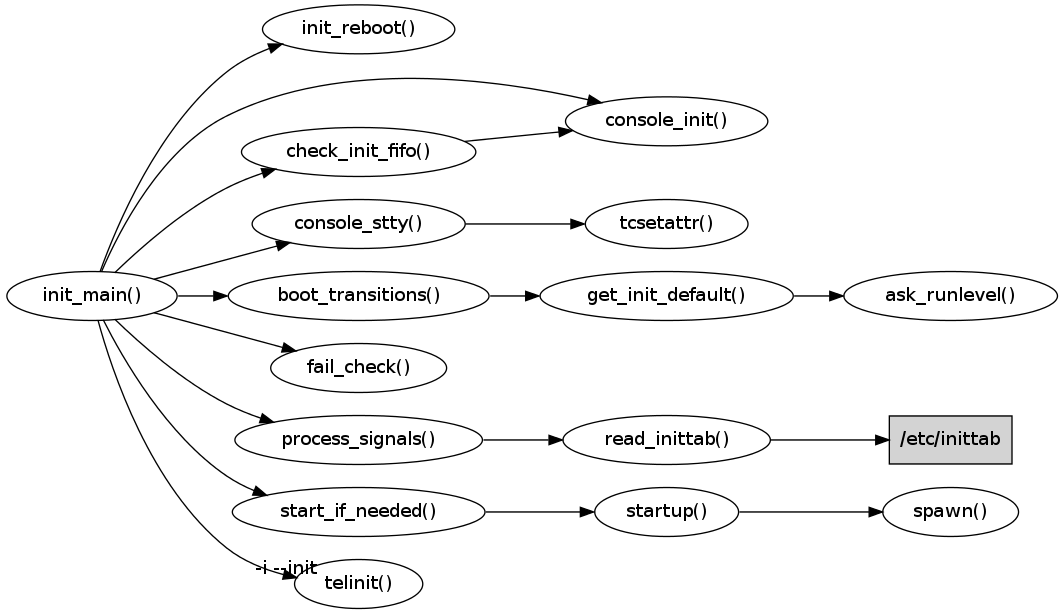
\includegraphics{./figures/init_main.png}
\caption{init\_main 函数核心代码}
\end{figure}

\subsection{console\_init 函数流程分析}

该函数主要完成的功能是: 设置 console\_dev 变量为一个可以工作的 console

函数执行流程分析:

{\begin{shaded}\begin{verbatim}
1. 获取 CONSOLE 环境变量的值,赋值给 console_dev 全局变量( char * 类型 )。

2. 以只读非阻塞方式打开 console_dev 所代表的设备文件。

3. 初始化成功,则关闭该设备文件;如果失败,则将 console_dev 置为 /dev/null 。
\end{verbatim}\end{shaded}}
\subsection{read\_inittab 函数流程分析}

该函数主要完成的功能是: 读取 /etc/inittab
文件,解析其中的约定规则,形成一个 CHILD 链表数据结构中。

该函数中用到的重要数据结构有 CHILD (struct \emph{child}) 和 actions 数组
(struct actions)

\subsubsection{CHILD 机构体 (struct \emph{child})}

这个链表数据结构在 init.h 头文件中,是实现根据 init
运行级别加载不同用户程序的最重要的数据结构。

{\begin{shaded}\begin{verbatim}
00082 /* Information about a process in the in-core inittab */
00083 typedef struct _child_ {
00084   int flags;                    /* Status of this entry */
00085   int exstat;                   /* Exit status of process */
00086   int pid;                      /* Pid of this process */
00087   time_t tm;                    /* When respawned last */
00088   int count;                    /* Times respawned in the last 2 minutes */
00089   char id[8];                   /* Inittab id (must be unique) */
00090   char rlevel[12];              /* run levels */
00091   int action;                   /* what to do (see list below) */
00092   char process[128];            /* The command line */
00093   struct _child_ *new;          /* New entry (after inittab re-read) */
00094   struct _child_ *next;         /* For the linked list */
00095 } CHILD;
00096 
\end{verbatim}\end{shaded}}
\subsubsection{actions 数组 (struct actions)}

这个数组保存的都是常量,包括常量字符串和宏定义,主要是一组对应关系,方便把
/etc/inittab 文件中的字符串转换为整型数。

例如 respawn -\textgreater{} RESPAWN, sysinit -\textgreater{} SYSINIT,
initdefault -\textgreater{} INITDEFAULT

{\begin{shaded}\begin{verbatim}
00150 
00151 /* ascii values for the `action' field. */
00152 struct actions {
00153   char *name;
00154   int act;
00155 } actions[] = {
00156   { "respawn",     RESPAWN      },
00157   { "wait",        WAIT         },
00158   { "once",        ONCE         },
00159   { "boot",        BOOT         },
00160   { "bootwait",    BOOTWAIT     },
00161   { "powerfail",   POWERFAIL    },
00162   { "powerfailnow",POWERFAILNOW },
00163   { "powerwait",   POWERWAIT    },
00164   { "powerokwait", POWEROKWAIT  },
00165   { "ctrlaltdel",  CTRLALTDEL   },
00166   { "off",         OFF          },
00167   { "ondemand",    ONDEMAND     },
00168   { "initdefault", INITDEFAULT  },
00169   { "sysinit",     SYSINIT      },
00170   { "kbrequest",   KBREQUEST    },
00171   { NULL,          0            },
00172 };
\end{verbatim}\end{shaded}}
\subsubsection{ACTIONS 宏定义}

这一组宏定义的值,也是保存在 init.h 头文件中。

{\begin{shaded}\begin{verbatim}
00065 /* Actions to be taken by init */
00066 #define RESPAWN                 1
00067 #define WAIT                    2
00068 #define ONCE                    3
00069 #define BOOT                    4
00070 #define BOOTWAIT                5
00071 #define POWERFAIL               6
00072 #define POWERWAIT               7
00073 #define POWEROKWAIT             8
00074 #define CTRLALTDEL              9
00075 #define OFF                    10
00076 #define ONDEMAND               11
00077 #define INITDEFAULT            12
00078 #define SYSINIT                13
00079 #define POWERFAILNOW           14
00080 #define KBREQUEST               15
\end{verbatim}\end{shaded}}
\subsubsection{read\_inittab 函数执行流程分析}

{\begin{shaded}\begin{verbatim}
1. 读取 /etc/inittab 文件,按行读取,到 buf 数组中。

2. 遇到开头是空格或者TAB制表符的行,忽略直到第一个字母,如果发现是第一个字母是#开头的注释,或者\n开头的空行,都直接跳过。

3. 使用 strsep 函数,以 : 冒号作为间隔符号,依次找到 id, rlevel, action, process 这4个字段,分别代表的含义可参考下面的详细说明。同时将 action 字段中的字符串关键字转换为整型数 actionNo,方便后面的判别。

4. 检查当前的 id 字段,是否是唯一的,如果之前已经出现过,则忽略掉。

5. 通过 imalloc 函数,动态分配 CHILD 结构体节点ch,结构体的定义见上面。然后将刚才分析的结果填入结构体中,并将这个节点,添加到链表 newFamily 中。其中包括 actionNo 填入 ch->action, id 填入 ch->id, process 填入 ch->process 等。

6. 关闭 /etc/inittab 文件。

7. 接下来,查看老的启动进程列表 family,看是否有进程需要被杀死的。这里有两轮检查,第一轮会给所有没有在新的运行级别中定义的进程发送一个警告信号 SIGTERM。如果在第一轮中有这样的进程,则会等待5秒,然后进入下一轮检查。在第2轮检查中,它会发送 SIGKILL 信号来强制中止所有子进程的运行。

8. 等所有子进程被杀死后,init 通过调用 write_utmp_wtmp() 来将终止信息和原因记录进这两个文件中。记录的信息包括子进程在 inittab 文件中的 id,子进程本身的 pid 等。

9. 这2个步骤7,8完成之后,init 开始清除老的 family 链表上的所有节点,释放空间。

10. 最后 init 把刚才新建成的 newFamily 链表赋值给 -> family 链表,完成重建链表的操作即结束。
\end{verbatim}\end{shaded}}
\subsection{start\_if\_needed 函数流程分析}

该函数主要完成的功能是: 遍历 family 链表,调用 startup
启动链表上的子进程。

函数执行流程分析:

{\begin{shaded}\begin{verbatim}
1. 从 family 链表的表头开始遍历该链表,根据每一个节点 ch 的 flags 标志来进行判别。

2. 如果当前节点 flags 表示 WAITING, 则说明正在等待,之前的工作未完成,立即退出该函数。

3. 如果当前节点 flags 表示 RUNNING, 则对这个正在运行的进程不做任何操作,继续下一个。

4. 如果当前节点的运行级别正好是当前 init 运行级别,则调用 startup 函数启动这个进程。

5. 如果当前节点不属于在当前运行级别中运行的程序,则将节点 flags 设置为 ~(RUNNING | WAITING) 表示不是运行中,也不是等待中。
\end{verbatim}\end{shaded}}
\subsection{startup 函数流程分析}

该函数主要完成的功能是: 执行 CHILD
节点所代表的配置行上的命令行,通常是个脚本程序。

函数执行流程分析:

{\begin{shaded}\begin{verbatim}
1. 对于 CHILD *ch 节点中的 action 字段来进行判别。如果是 SYSINIT,BOOTWAIT,WAIT,POWERWAIT,POWERFAILNOW,POWEROKWAIT,CTRLALTDEL 这些情况,则设置标志为 WAITING,然后执行 spawn 函数。这个函数是完成启动子进程的真正的函数,spawn 名字的含义是产卵的意思,顾名思义就是产生后继的子进程。后面我们再对这个函数做详细分析。

2. 如果是 KBREQUEST,BOOT,POWERFAIL,ONCE 则直接退出,不进行后继的 spawn 函数调用。

3. 如果是 ONDEMAND,RESPAWN,则将 flags 设置为 RUNNING 后,立即执行 spawn 操作。
\end{verbatim}\end{shaded}}
\subsection{spawn 函数流程分析}

该函数主要完成的功能是: 调用 fork 和 execp
来启动子进程。这个函数非常长,但基本上是属于最底层的函数了。

函数执行流程分析:

{\begin{shaded}\begin{verbatim}
1. spawn 整个程序比较长,从927-1192行约有270多行。整个代码逻辑以 fork 调用为分界线,可以分为2个部分。前面部分主要完成启动前的准备工作,后面通过 fork 和 execp 来实际创建出子进程执行 CHILD 节点上规定的程序。

2. 先分析第一部分。这部分代码主要处理三种情况,1是action 为“RESPAWN”与“ONDEMAND”类型的命令;2是 /etc/initscript 初始化脚本为后继 execp 调用准备参数。

3. 第二部分进入到一个无限循环中,以便确保能够成功创建出子进程。在调用 fork 创建出 init 的子进程之后,init 的这个子进程将按照 daemon 进程的方式工作,包括需要关闭0,1,2打开文件。也就是说,真正用来创建用户子进程的,不是 pid = 1 的那个原始进程,而是原始进程的子进程再通过一个 fork 和 execp 才能够实现执行真正的用户程序。

4. 第2次执行 fork 之后,由子进程调用 execp 来完成加载用户程序,而父进程通过调用 waitpid 来等待子进程的结束。

5. 上述步骤完成之后,父进程又会创建出一个临时的子进程,来完成 setsid() 和 ioctl(f, TIOCSCTTY, 1) 这2个函数调用,来分配一个控制终端,创建一个新的会话,失去原有的控制终端的所有联系。
\end{verbatim}\end{shaded}}
\subsection{boot\_transitions 函数流程分析}

该函数主要完成的功能是:
实现一个启动过程中所需要的状态机,完成状态的迁移。

函数执行流程分析:

{\begin{shaded}\begin{verbatim}
1. 以 runlevel 代表状态,如果当前 runlevel = '#' 状态开始,系统进入 SYSINIT -> BOOT 的转变。

2. 如果在 read_inittab 时从文件中获得了 def_level,则直接用这个变量的值,否则通过 get_init_default() 得到的是默认的运行级别并赋值给 newlevel

3. 如果 newlevel 是 'S', 则下一个状态为 'S',否则下一个状态设为 '*'

4. 如果当前 runlevel 是 '*',则系统从 BOOT -> NORMAL。

5. 如果当前 runlevel 是 'S',则代表着 SU 模式已经结束,重新调用 get_init_default() 得到新的运行级别 newlevel.

6. 将本次状态变迁的信息写入日志 write_utmp_wtmp()
\end{verbatim}\end{shaded}}
\subsection{check\_init\_fifo() 函数流程分析}

该函数主要完成的功能是: 主要用于 init daemon 程序中,通过 select
函数监听来自于 /dev/initctl 管道的请求 request,分析并执行该请求
request。

函数执行流程分析:

{\begin{shaded}\begin{verbatim}
1. 如果 /etc/initctl 管道不存在,则创建这个管道,并设置权限 0600,只允许 root 用户读写。

2. 如果管道已经打开,则比较该管道是否是最初原始打开的管道。如果不是,则关闭后,重新打开。

3. 以读写+非阻塞方式打开管道,并且使用 dup2 将采用 PIPE_FD = 10 来使用管道,而不使用 0,1,2

4. 使用 select 调用在该管道上等待来自于 init N 的切换运行级别的请求 request

5. 一旦有来自这个管道的 request ,则检查这个 request 数据的合法性

6. 对于输入正确的 request 请求,则分析是什么请求,并判断要采取什么动作。

7. 请求包括进行 
    INIT_CMD_RUNLVL (runlevel 的切换) -> 调用 fifo_new_level()
    INIT_CMD_POWERFAIL
    INIT_CMD_POWERFAILNOW
    INIT_CMD_POWEROK (以上三个请求都是和电源事件有关)  -> 调用 do_power_fail()
    INIT_CMD_SETENV (设置环境变量) -> 调用 initcmd_setenv()
\end{verbatim}\end{shaded}}
\subsubsection{struct init\_request 请求协议格式}

通过 /etc/initctl 管道
进行请求的数据,需要遵循一定的格式,也就是需要能够转换为如下的
init\_request 结构体数据。

{\begin{shaded}\begin{verbatim}
00073 struct init_request {
00074         int     magic;                  /* Magic number                 */
00075         int     cmd;                    /* What kind of request         */
00076         int     runlevel;               /* Runlevel to change to        */
00077         int     sleeptime;              /* Time between TERM and KILL   */
00078         union {
00079                 struct init_request_bsd bsd;
00080                 char                    data[368];
00081         } i;
00082 };
00083 
\end{verbatim}\end{shaded}}
\subsubsection{cmd 请求类别标识}

所有正确的请求,都有一个唯一的标识,这些标识定义在 initreq.h 头文件中。

{\begin{shaded}\begin{verbatim}
00035 #define INIT_CMD_START          0
00036 #define INIT_CMD_RUNLVL         1
00037 #define INIT_CMD_POWERFAIL      2
00038 #define INIT_CMD_POWERFAILNOW   3
00039 #define INIT_CMD_POWEROK        4
00040 #define INIT_CMD_BSD            5
00041 #define INIT_CMD_SETENV         6
00042 #define INIT_CMD_UNSETENV       7
\end{verbatim}\end{shaded}}
\subsection{fail\_check 函数流程分析}

该函数主要完成的功能是: 在每次信号处理完成之后,遍历 family
链表检查每个节点的状态

函数执行流程分析:

{\begin{shaded}\begin{verbatim}
1. 首先调用 time(&t) 获得系统时间。

2. 从 family 链表头开始,遍历整个链表,直到结束。 

3. 检查每一个节点 ch 的 flags 是否表示 FAILING

4. 如果是,并且这个进程已经睡眠 sleep 了至少5分钟,则会清除掉  flags 中的 FAILING 标识位。

5. 如果不是,则设置下一次 alarm 的时间为这个进程 sleep 的时间加上 5 分钟。
\end{verbatim}\end{shaded}}
\subsubsection{SLEEEPTIME 数据}

睡眠时间超过300秒=5分钟的进程,将会被清除标志位

{\begin{shaded}\begin{verbatim}
#define SLEEPTIME   300
\end{verbatim}\end{shaded}}
\subsection{process\_signals 函数流程分析}

该函数主要完成的功能是: 根据全局变量 got\_signals
中哪些标志位被设置了,获得信号类型,进行相应的处理。

函数执行流程分析:

{\begin{shaded}\begin{verbatim}
程序执行逻辑很简单,就是依次判别 ISMEMBER(got_signals, SIGXXXX) 对于以下信号进行相应处理。

1. SIGPWR 信号 -> do_power_fail()

2. SIGINT 信号 -> 通知 ctrlaltdel 入口启动

3. SIGWINCH 信号 -> 通知 KBREQUEST 入口启动

4. SIGALRM 信号 -> 定时器到时,忽略

5. SIGCHLD 信号 -> 查看是哪个子进程结束,调用 write_utmp_wtmp() 写入日志

6. SIGHUP 信号 -> 是否在等待子进程,进行 runlevel 切换

7. SIGUSR1 信号 -> 这个信号代表要求关闭然后重新打开 /dev/initctl
\end{verbatim}\end{shaded}}
在 set.h 头文件中有关于这个宏定义的实现

{\begin{shaded}\begin{verbatim}
#define     ISMEMBER(set, val)   ((set) & (1 << (val)))
#define     DELSET(set, val)   ((set) &= ~(1 << (val)))
#define     ADDSET(set, val)   ((set) |= (1 << (val)))
#define     EMPTYSET(set)   ((set) = 0)
\end{verbatim}\end{shaded}}
通过 kill -l 可以得到这些 SIGXXXX 的具体赋值,如下:

{\begin{shaded}\begin{verbatim}
$ kill -l
 1) SIGHUP   2) SIGINT   3) SIGQUIT  4) SIGILL   5) SIGTRAP
 6) SIGABRT  7) SIGBUS   8) SIGFPE   9) SIGKILL 10) SIGUSR1
11) SIGSEGV 12) SIGUSR2 13) SIGPIPE 14) SIGALRM 15) SIGTERM
16) SIGSTKFLT   17) SIGCHLD 18) SIGCONT 19) SIGSTOP 20) SIGTSTP
21) SIGTTIN 22) SIGTTOU 23) SIGURG  24) SIGXCPU 25) SIGXFSZ
26) SIGVTALRM   27) SIGPROF 28) SIGWINCH    29) SIGIO   30) SIGPWR
31) SIGSYS  34) SIGRTMIN    35) SIGRTMIN+1  36) SIGRTMIN+2  37) SIGRTMIN+3
38) SIGRTMIN+4  39) SIGRTMIN+5  40) SIGRTMIN+6  41) SIGRTMIN+7  42) SIGRTMIN+8
43) SIGRTMIN+9  44) SIGRTMIN+10 45) SIGRTMIN+11 46) SIGRTMIN+12 47) SIGRTMIN+13
48) SIGRTMIN+14 49) SIGRTMIN+15 50) SIGRTMAX-14 51) SIGRTMAX-13 52) SIGRTMAX-12
53) SIGRTMAX-11 54) SIGRTMAX-10 55) SIGRTMAX-9  56) SIGRTMAX-8  57) SIGRTMAX-7
58) SIGRTMAX-6  59) SIGRTMAX-5  60) SIGRTMAX-4  61) SIGRTMAX-3  62) SIGRTMAX-2
63) SIGRTMAX-1  64) SIGRTMAX    
$ 
\end{verbatim}\end{shaded}}
\subsection{console\_stty 函数流程分析}

该函数主要完成的功能是: 设置终端工作参数

函数执行流程分析:

{\begin{shaded}\begin{verbatim}
1. 调用 console_open 打开 console_dev 设备,模式为读写+非阻塞方式。

2. 调用 tcgetattr() 函数获得当前终端属性 tty (struct termios 结构体)

3. 设置 tty.c_cflag 和 tty.c_cc[] 的参数配置。

4. 设置 tty.c_iflag 和 tty.c_oflag 以及 tty.c_lflag 参数配置。

5. 调用 tcsetattr() 和 tcflush() 完成设置终端属性的操作。

6. 调用 close(fd) 关闭终端设备文件。
\end{verbatim}\end{shaded}}
\subsection{fifo\_new\_level 函数流程分析}

该函数主要完成的功能是: 真正完成改变 runlevel 的 request
请求,目标为传入参数 level,通过重新读取 inittab 文件来启动与新 runlevel
匹配的命令脚本。

函数执行流程分析:

{\begin{shaded}\begin{verbatim}
1. 如果传入参数 level 和当前的 runlevel 运行级别一致,则无需修改直接返回。

2. 如果新的 runlevel = 'U',则通过调用 re_exec() 来执行改变 runlevel 的操作。

3. 如果新的 runlevel != 'U',则通过调用 read_inittab() 来重新生成 family 链表。
\end{verbatim}\end{shaded}}
\subsection{re\_exec 函数流程分析}

该函数主要完成的功能是: 强制 init 程序重新执行。

函数执行流程分析:

{\begin{shaded}\begin{verbatim}
1. 该函数会创建 STATE_PIPE,并向 STATE_PIPE 写入 Signature = "12567362"

2. 接着fork()出一个子进程,通过子进程调用 send_state() 向 STATE_PIPE 写入父进程(当前init进程)的状态信息;

3. 然后父进程调用 execle() 重新执行 init 程序,并且传递参数“--init”, 也就是强制init重新执行。而这个重新执行的 init 进程,无需做初始化读取 /etc/inittab 就能调用 init_main()。
\end{verbatim}\end{shaded}}
\subsection{get\_init\_default 函数流程分析}

该函数主要完成的功能是: 查找 /etc/inittab 文件中的 initdefault
默认运行级别,如果有则返回,如果没有则请用户输入。

函数执行流程分析:

{\begin{shaded}\begin{verbatim}
1. 实际上这个函数是从 family 链表中遍历,取出每一个节点 ch

2. 如果 ch->action == INITDEFAULT ,则将当前 ch 的运行级别赋值给 lvl

3. 判断如果 lvl 是小写,则转换为大写。并且对 lvl 进行判别,看它是否属于 “0123456789S“ 的其中之一。

4. 如果从文件中得到的 lvl 正确,则返回 lvl; 

5. 如果从文件中无法得到正确的 lvl,则调用 ask_runlevel() 函数返回。这个函数中会通过终端来询问用户,并要求用户输入一个默认运行级别。
\end{verbatim}\end{shaded}}
\subsection{telinit 函数流程分析}

在执行 telinit
函数时,实际上是通过向INIT\_FIFO(/dev/initctl)写入命令的方式,通知 init
执行相应的操作。Telinit()根据不同请求,构造如下结构体类型的变量并向INIT\_FIFO(/dev/initctl)写入该请求来完成其使命:

struct init\_request \{ int magic; /* Magic number \emph{/ int cmd; /}
What kind of request \emph{/ int runlevel; /} Runlevel to change to
\emph{/ int sleeptime; /} Time between TERM and KILL */ union \{ struct
init\_request\_bsd bsd; char data{[}368{]}; \} i; \};

\section{init进程执行流程分析}

通过以上这些子函数的分析,我们可以总结一下关于 init
进程的运行状态和相应的执行流程。

\subsection{init程序的3种启动执行方式}

\subsection{方式1 - Kernel 启动 init}

在内核启动代码中,start\_kernel 函数初始化代码的结束,会通过 command\_line
来找出 init=execute\_command 字符串中的程序来执行,或者按照默认的4个 init
程序的顺序依次来调用 execve() 执行 init 进程。这种方式启动的 init
进程,会完成读取 /etc/inittab 文件,建立 family
链表,依次执行各个子进程,并等待子进程的结束。当 init
进程运行到最后会进入一个无限循环中,变成一个 daemon init 进程。

这种启动方式,也是在整个操作系统启动过程中,init
程序的初次执行。这种启动是在内核空间启动 init 。

\begin{figure}[htbp]
\centering
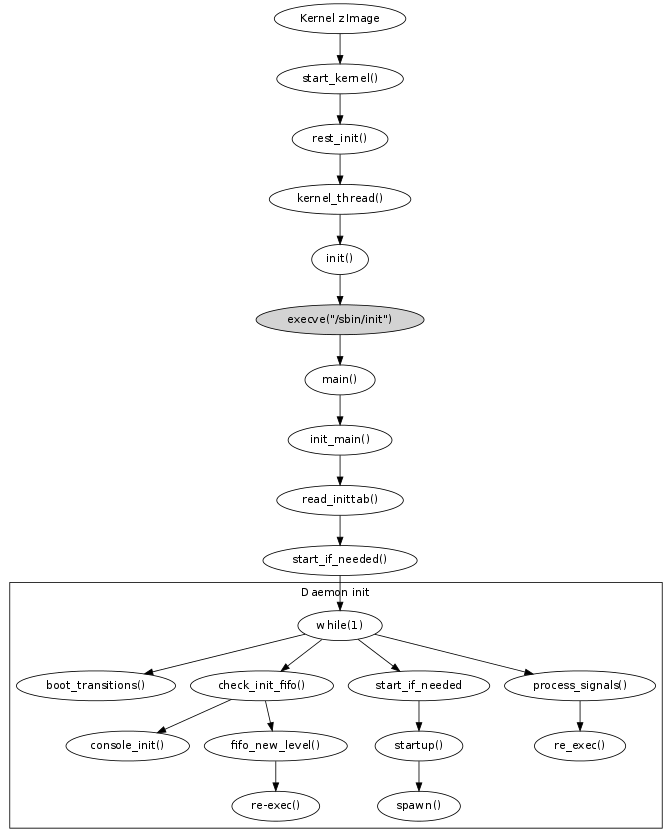
\includegraphics{./figures/how-to-exec-init-1.png}
\caption{方式1 - Kernel 启动 init}
\end{figure}

\subsection{方式2 - 用户命令 telinit 启动 init}

在 init 进程启动之后,用户通过终端可以完成登录进入 Bash 中,执行 telinit
命令的时候,因为 telinit 命令本身就是一个指向 init
程序的软链接,所以会导致 init 程序再次被执行。通过这种方式运行起来的 init
进程,因为 pid != 1 因此可以判断不是 Kernel 创建的 init
进程,此时会转为调用 telinit() 函数来执行。

这种情况下,telinit() 函数只负责打开 INIT\_FIFO(/dev/initctl)
并按照传入参数,组织为一个 struct request 结构体,写入 FIFO
中,通知方式1中的 init 进程,就完成任务了。

这种启动方式通常会涉及到 runlevel 的切换,例如执行 telinit 1 或者 init 1
就会引起系统切换到单用户模式下。这是 init
程序的第2种常用的启动方式。我们可以看成是在用户空间启动 init 。

\begin{figure}[htbp]
\centering
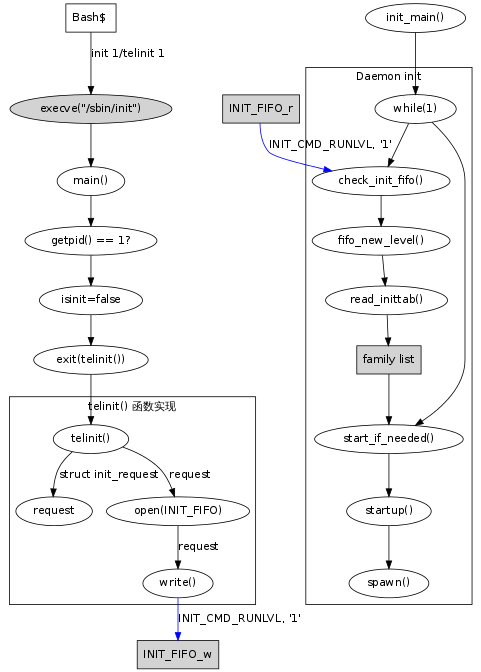
\includegraphics{./figures/how-to-exec-init-2.png}
\caption{方式2 - 用户命令 telinit 启动 init}
\end{figure}

\subsection{方式3 - 在程序中通过 re\_exec() 函数启动 init}

这种方式发生在通过方式1启动了init之后,在 init
执行的最后,进入了一个无限循环等待中。此时,用户如果在终端下执行 telinit U
命令,则代表着用户希望 re-execute itself,那么在方式2启动 init 之后,新的
init 进程会发送 U 命令给方式1启动的 init
进程,这个最原始的进程在循环中会调用 process\_signals() 来处理 U
命令,处理方法是调用 re\_exec() 函数。在这个函数中,会 fork
出一个子进程,子进程通过管道向父进程发送消息,由父进程通过 execle()
重新执行 init 程序,并传递 --init 参数,强制 init 重新执行。

和方式1的执行所不同的是,方式1在执行的后期,会读取 /etc/inittab 文件,建立
family 链表;而方式3因为是用户通过 telinit U 的方式告诉 方式1启动的那个
daemon init 进程,调用 re\_exec() 函数,因此最原始的那个 init
进程,不会进行之前的 read\_inittab()
初始化操作,而是直接进入到无限循环,又一次进入 daemon 的等待/处理循环中。

\begin{figure}[htbp]
\centering
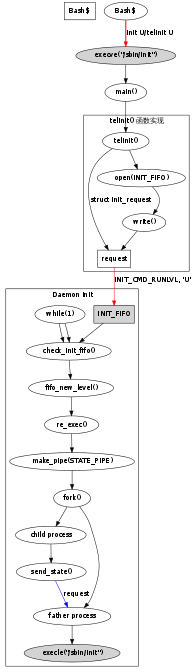
\includegraphics{./figures/how-to-exec-init-3.png}
\caption{方式3 - 在程序中通过 re\_exec() 函数启动 init}
\end{figure}

\subsection{三种方式的相互联系}

我们用一张总图来表示上述3种启动 init 的方式之间的相互联系。

\begin{figure}[htbp]
\centering
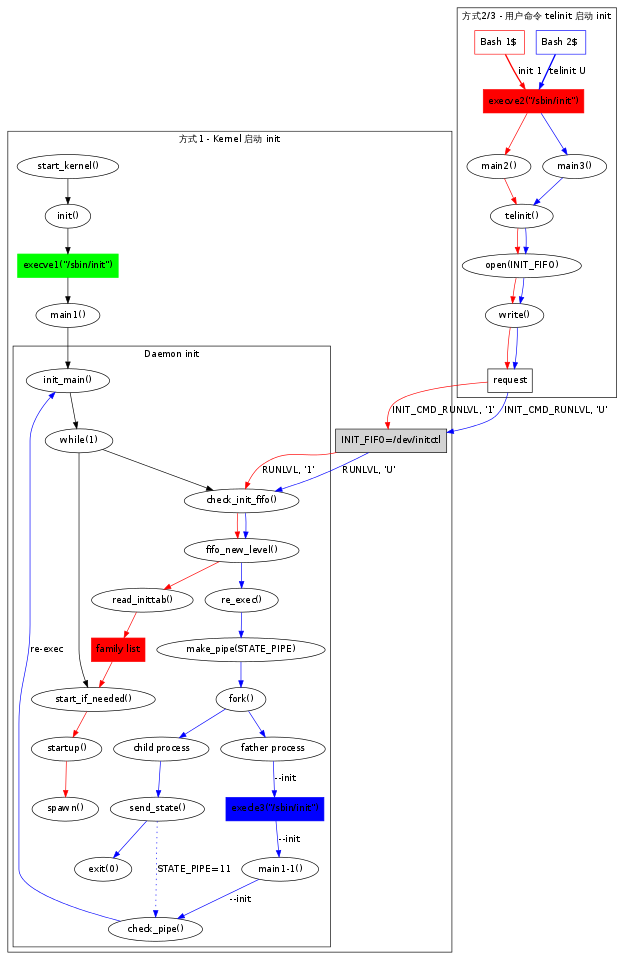
\includegraphics{./figures/how-to-exec-init.png}
\caption{方式1,2,3的相互联系}
\end{figure}

\begin{itemize}
\item
  图中红色部分的线路表示方式2和方式1之间的联系。
\item
  图中蓝色部分的线路表示方式3和方式1之间的联系。
\item
  方式2和3之间没有通信。
\item
  相同点
  \begin{itemize}
  \item
    方式2和3都是通过 Bash 命令启动 init 进程。
  \item
    方式2和3都是通过 INIT\_FIFO 来和 Daemon init 进程进行通信。
  \end{itemize}
\item
  不同点,方式2和3传递的参数不同。
  \begin{itemize}
  \item
    方式2主要是传递新的优先级,例如 init 1, 表示要切换 init
    进程到新的优先级1上工作。
  \item
    方式3主要是要求重新启动init进程,并不需要修改优先级,例如 telinit U。
  \end{itemize}
\end{itemize}
\subsection{三种方式的比较区别}

\begin{itemize}
\item
  通过方式1启动的 init 进程 pid=1。
\item
  通过方式2和3启动的 init 进程,pid 一定不是 1 ,所以这个进程和前面的这个
  init
  进程完全不同。它们是分别属于内核空间和用户空间的2个不同的进程(前者进程1其实应该称为内核线程,因为它是通过
  kernel\_thread() 创建出来的,而后者是通过 shell 在用户空间 fork
  出来的,是真正的用户程序,只不过这个用户程序只做了一个向管道发送数据的操作。
\item
  通过方式3,又让 pid=1 的原始 init 进程调用了 re\_exec() -\textgreater{}
  fork() -\textgreater{} execle() 来(让父进程pid=1)重新加载了一次的 init
  进程,本质上其实都是 1 号进程。但 fork() 出的子进程,其实也算是一个 init
  进程,只不过它只完成了向父进程的 STATE\_PIPE 写一下状态信息就退出
  exit(0) 了,生命期很短。
\item
  方式2和3虽然启动的参数不一样,但都是通过调用 telinit 函数,对 INIT\_FIFO
  进行写 request 的操作。
  \begin{itemize}
  \item
    两者的 request 参数略有不同
  \item
    request.cmd 都是 INIT\_CMD\_RUNLVL
  \item
    request.runlevel 则 一个是 `1', 一个是 `U'
  \item
    在 fifo\_new\_level() 函数中,有对这2者的不同处理,前者调用
    read\_inittab(), 后者调用 re\_exec()。
  \end{itemize}
\end{itemize}
因此程序从 fifo\_new\_level() 函数这里开始有了不同的分支流程。

\begin{itemize}
\item
  方式2会沿着红色线路,执行流程如下
  \begin{itemize}
  \item
    调用 read\_inittab() -\textgreater{} 更新 family 链表
  \item
    在 Daemon 循环中,从 start\_if\_needed() -\textgreater{} startup()
  \item
    最后通过 spawn() 完成启动 inittab 文件中的子进程。
  \end{itemize}
\item
  方式3会沿着蓝色线路,执行流程如下
  \begin{itemize}
  \item
    调用 re\_exec() -\textgreater{} make\_pipe(STATE\_PIPE)
    创建管道(fd=11)
  \item
    然后通过 fork() 分出1个子进程,这个子进程只负责给父进程 STATE\_PIPE
    管道发送状态信息
  \item
    父进程紧接着通过 execle() 来重新启动 init 进程,并传递一个启动参数
    --init,使得再次启动 init 进程的时候,isinit=1。
  \item
    这时父进程会进入 check\_pipe() 函数中检查管道 STATE\_PIPE
    中是否有数据,是否符合要求。
  \item
    如符合,则设置 reload=1,调用 init\_main() 再次进入 Deamon 状态。
  \item
    这一次进入 Daemon 之前,只需要执行 start\_if\_needed 而无需执行
    read\_inittab(),也就是不需要再重新读取 /etc/inittab 文件。这是
    re\_exec 方式3和 Kernel 启动 init 方式1 之间的最大区别。
  \end{itemize}
\end{itemize}
\section{halt命令执行流程分析}

\subsection{halt 命令的数据分析}

根据 halt 命令的参数,在 main 函数的实现中,引入了如下这些变量。

{\begin{shaded}\begin{verbatim}
00177         int do_reboot = 0;
00178         int do_sync = 1;
00179         int do_wtmp = 1;
00180         int do_nothing = 0;
00181         int do_hard = 0;
00182         int do_ifdown = 0;
00183         int do_hddown = 0;
00184         int do_poweroff = 0;
\end{verbatim}\end{shaded}}
\subsection{halt命令实现代码分析}

\subsubsection{参数解析}

从下面的 switch-case 语句分支中,可以很清楚的看出 halt
命令参数和上述变量之间的对应关系。

{\begin{shaded}\begin{verbatim}
progname = argv[0];

00198         if (!strcmp(progname, "reboot")) do_reboot = 1;
00199         if (!strcmp(progname, "poweroff")) do_poweroff = 1;
00200 
00201         /*
00202          *      Get flags
00203          */
00204         while((c = getopt(argc, argv, ":ihdfnpwt:")) != EOF) {
00205                 switch(c) {
00206                         case 'n':
00207                                 do_sync = 0;
00208                                 do_wtmp = 0;
00209                                 break;
00210                         case 'w':
00211                                 do_nothing = 1;
00212                                 break;
00213                         case 'd':
00214                                 do_wtmp = 0;
00215                                 break;
00216                         case 'f':
00217                                 do_hard = 1;
00218                                 break;
00219                         case 'i':
00220                                 do_ifdown = 1;
00221                                 break;
00222                         case 'h':
00223                                 do_hddown = 1;
00224                                 break;
00225                         case 'p':
00226                                 do_poweroff = 1;
00227                                 break;
00228                         case 't':
00229                                 tm = optarg;
00230                                 break;
00231                         default:
00232                                 usage();
00233                 }
00234          }
\end{verbatim}\end{shaded}}
\subsubsection{不同参数对应着不同处理}

后继的代码很简单,就是根据不同的参数,进行不同的函数调用来处理。我们用一张图来表示:

\begin{figure}[htbp]
\centering
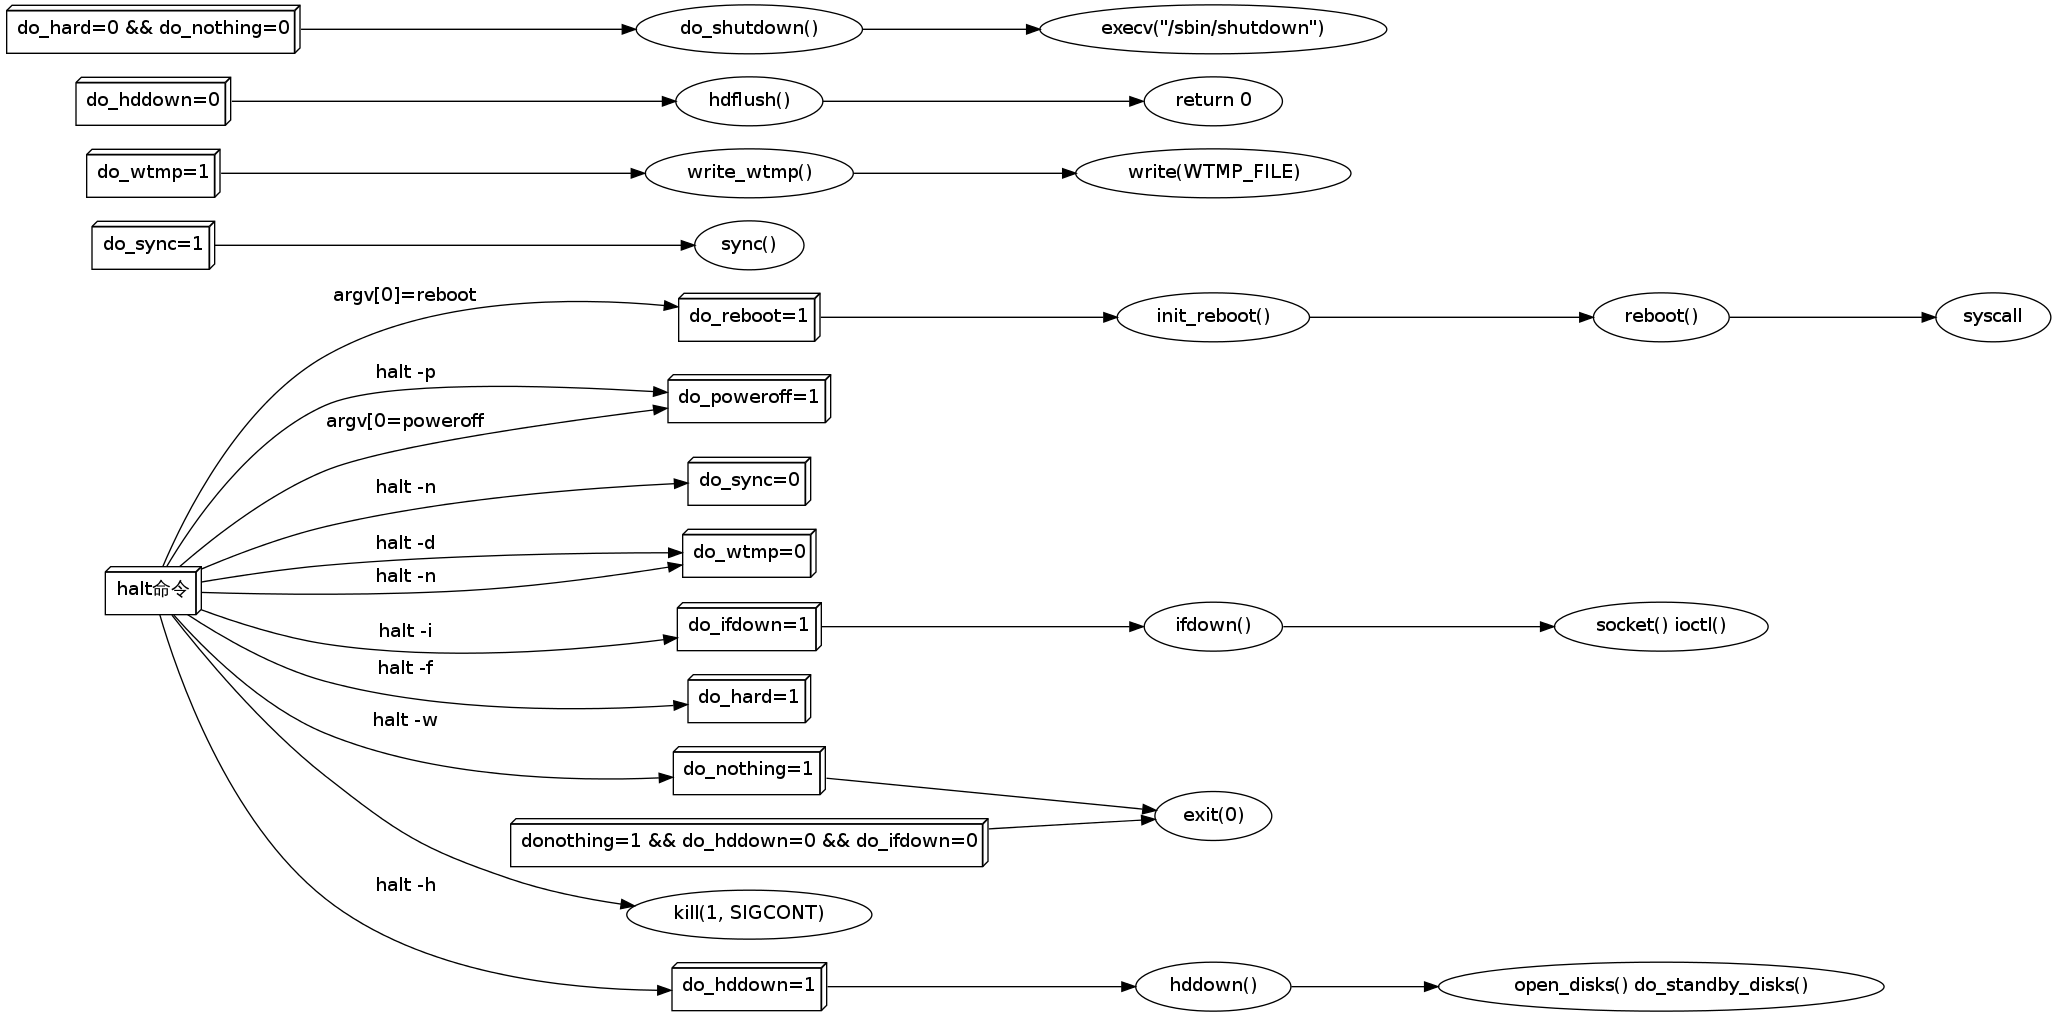
\includegraphics{./figures/halt.png}
\caption{halt命令参数及相应处理函数流程}
\end{figure}

从图中可以看出:

\begin{itemize}
\item
  reboot 是 halt 命令的软链接
\item
  poweroff 是 halt 命令的软链接,等价于 halt -p
\item
  halt 命令是依靠 execv(``/sbin/shutdown'') 调用 shutdown
  命令来完成工作的。
\item
  shutdown 命令是关机的核心命令,其他命令都不如这个命令重要。
\end{itemize}
\section{shutdown命令执行流程分析}

\subsection{shutdown命令的数据分析}

\subsection{shutdown命令实现代码分析}

shutdown 的核心代码在 shutdown() 函数中,除了用 openlog(), syslog(),
closelog() 来写关机日志外,主要是靠调用 execv(INIT, args) 来启动 init
进程完成改变运行级别的工作,从而间接完成关机操作。

\section{sulogin命令执行流程分析}

\subsection{sushell函数代码分析}

该函数主要完成的功能是: 当用户的密码验证通过后,启动一个shell
(由环境变量SUSHELL指定)

函数执行流程分析:

{\begin{shaded}\begin{verbatim}
1. 调用 chdir 改变根目录

2. 调用 getenv 获取环境变量 SUSHELL 的值,并赋值给 sushell 指针

3. 设置一些环境变量 HOME,LOGNAME,USER 的值

4. 安装一些信号处理函数 SIGINT,SIGTSTP,SIGQUIT

5. 调用 execl 来执行 sushell 命令,如果失败,则依次执行 /bin/sh,/bin/sash
\end{verbatim}\end{shaded}}
\subsection{getrootpwent函数代码分析}

该函数主要完成的功能是: 获得根用户 root 的密码

函数执行流程分析:

{\begin{shaded}\begin{verbatim}
1. 首先通过标准的方法,使用普通库函数 getpwnam() 和 getspnam() 来获得密码,如果能找到则返回 pw

2. 如果找不到,则接下来尝试通过读取 passwd 和 shadow 文件手工来分析。

3. 读取 /etc/passwd 找到 root: 字符串开头的那行,如果没有这一行,则返回 root 密码为空

4. 如果有则调用 valid() 函数进行验证,验证成功,则返回 &pwd

5. 验证不成功,再检查 /etc/shadow 文件,如果有则返回 &pwd,如果没有则返回 空串。
\end{verbatim}\end{shaded}}
\subsection{getpasswd 函数代码分析}

该函数主要完成的功能是: 从标准输入获得用户输入的密码

函数执行流程分析:

{\begin{shaded}\begin{verbatim}
1. 打印提示信息,要求用户输入密码

2. 修改终端属性,不进行回显 NO echo

3. 注册信号 SIGALRM 的处理函数,以便能够超时处理

4. 从标准输入读取用户输入的密码字符串,存放在静态变量 static char pass[128] 数组中

5. 修改终端属性,恢复回显功能 echo,返回数组首地址
\end{verbatim}\end{shaded}}
\section{runlevel命令执行流程分析}

\subsection{utmpname 函数代码分析}

该函数主要完成的功能是: 设置utmp 文件路径

utmpname()用来设置utmp文件的路径,以提供utmp相关函数的存取路径。如果没有使用utmpname()则默认utmp文件路径为/var/run/utmp。

\subsection{setutent 函数代码分析}

该函数主要完成的功能是: 从头读取utmp 文件中的登录数据

setutent()用来将getutent()的读写地址指回utmp文件开头。

\subsection{getutent 函数代码分析}

该函数主要完成的功能是: 从utmp 文件中取得账号登录数据

getutent()用来从utmp 文件(/var/run/utmp)中读取一项登录数据,该数据以utmp
结构返回。第一次调用时会取得第一位用户数据,之后每调用一次就会返回下一项数据,直到已无任何数据时返回NULL。

\subsection{utmp结构定义}

{\begin{shaded}\begin{verbatim}
struct utmp
{
    short int ut_type;      /* 登录类型 */
    pid_t ut_pid;           /* login进程的pid */
    char ut_line[UT_LINESIZE];  /* 登录装置名,省略了/dev/ */
    char ut_id[4];          /* Inittab ID */
    char ut_user[UT_NAMESIZE];  /* 登录账号 */
    char ut_host[UT_HOSTSIZE];  /* 登录账号的远程主机名称 */
    struxt exit_status ut_exit; /* 当类型为DEAD_PROCESS时进程的结束状态 */
    long int ut_session;        /* Sessioc ID */
    struct timeval ut_tv;       /* 时间记录 */
    int32_t ut_addr_v6[4];      /* 远程主机的网络地址 */
    char __unused[20];      /* 保留未使用 */
};
\end{verbatim}\end{shaded}}
\subsubsection{ut\_type有以下几种类型}

{\begin{shaded}\begin{verbatim}
  EMPTY 此为空的记录。

  RUN_LVL 记录系统run-level的改变

  BOOT_TIME 记录系统开机时间

  NEW_TIME 记录系统时间改变后的时间

  OLD_TINE 记录当改变系统时间时的时间。

  INIT_PROCESS 记录一个由init衍生出来的进程。

  LOGIN_PROCESS 记录login进程。

  USER_PROCESS 记录一般进程。

  DEAD_PROCESS 记录一结束的进程。

  ACCOUNTING 目前尚未使用。
\end{verbatim}\end{shaded}}
\subsection{endutent 函数}

该函数主要完成的功能是: 关闭utmp 文件

endutent()用来关闭由getutent所打开的utmp文件。

\section{killall5 命令执行流程分析}

killall5 是 sysvinit 工具软件包中,从实现代码量上是仅次于 init
命令的一个重要命令。 下面我们从 killall5.c 文件的 main
函数开始分析整个命令的执行流程。

\subsection{killall5 主函数代码分析}

\subsubsection{获得执行程序名 progname}

{\begin{shaded}\begin{verbatim}
00986 /* Main for either killall or pidof. */
00987 int main(int argc, char **argv)
00988 {
00989         PROC            *p;
00990         int             pid, sid = -1;
00991         int             sig = SIGKILL;
00992         int             c;
00993 
00994         /* return non-zero if no process was killed */
00995         int             retval = 2;
00996 
00997         /* Get program name. */
00998         if ((progname = strrchr(argv[0], '/')) == NULL)
00999                 progname = argv[0];
01000         else
01001                 progname++;
01002 
\end{verbatim}\end{shaded}}
通过最开始一段代码,可以看出 sig = SIGKILL 默认的发送信号是
SIGKILL,这个信号是9号,默认处理动作是 exit。 progname
字符串指针是一个全局变量,经过赋值之后,获得了正在运行程序的名字,只是文件名,不包含路径名。

{\begin{shaded}\begin{verbatim}
00133 char *progname; /* the name of the running program */
\end{verbatim}\end{shaded}}
\subsubsection{打开系统日志}

下面这段代码是调用 openlog() 函数来打开以 progname
为日志文件名的日志文件。

{\begin{shaded}\begin{verbatim}
01003         /* Now connect to syslog. */
01004         openlog(progname, LOG_CONS|LOG_PID, LOG_DAEMON);
01005 
\end{verbatim}\end{shaded}}
\subsubsection{处理 pidof 命令的情况}

因为 pidof 是指向 killall5 的软链接,因此程序需要判断是通过执行 killall5
命令启动的,还是 pidof 命令启动的。 如果是 pidof 命令,则调用 main\_pidof
的主函数来实现这个命令,并在执行完 main\_pidof()
函数后直接返回,不再执行后继的代码。同时这个函数的返回值,也作为整个程序的返回值。

{\begin{shaded}\begin{verbatim}
01006         /* Were we called as 'pidof' ? */
01007         if (strcmp(progname, "pidof") == 0)
01008                 return main_pidof(argc, argv);
\end{verbatim}\end{shaded}}
因为 pidof
命令在下面我们专门有一个小节来讨论,因此我们不在此展开,而是继续接着
killall5 命令的执行流程分析下去。

\subsubsection{分析 -o omitpid 参数创建双向链表 omit}

程序进行到此,确定是用户要执行 killall5 命令。同时给 omit 链表赋值为 0
,表示此时链表为空。

{\begin{shaded}\begin{verbatim}
01010         /* Right, so we are "killall". */
01011         omit = (OMIT*)0;
01012 
\end{verbatim}\end{shaded}}
下面是开始进行传入参数的匹配处理。因为 killall5 命令支持 -o 参数传递
omitpid ,也就是可以被忽略的进程不进行 kill 操作,因此要取出 argv{[}{]}
参数列表中的所有 omitpid 。

从代码中可以看出,strsep(\&hear, ``,;:'')
其中以逗号,分号,冒号作为分隔符,以 omit 为链表头,不断分析 argv{[}{]}
数组中和 -o 有关的 pid 列表,然后负责用动态生成节点的方式,创建链表。

{\begin{shaded}\begin{verbatim}
01013         if (argc > 1) {
01014                 for (c = 1; c < argc; c++) {
01015                         if (argv[c][0] == '-') (argv[c])++;
01016                         if (argv[c][0] == 'o') {
01017                                 char * token, * here;
01018 
01019                                 if (++c >= argc)
01020                                         usage();
01021 
01022                                 here = argv[c];
01023                                 while ((token = strsep(&here, ",;:"))) {
01024                                         OMIT *restrict optr;
01025                                         pid_t opid = (pid_t)atoi(token);
01026 
01027                                         if (opid < 1) {
01028                                                 nsyslog(LOG_ERR,
01029                                                         "illegal omit pid value "
01030                                                         "(%s)!\n", token);
01031                                                 continue;
01032                                         }
01033                                         xmemalign((void*)&optr, sizeof(void*), alignof(OMIT));
01034                                         optr->next = omit;
01035                                         optr->prev = (OMIT*)0;
01036                                         optr->pid  = opid;
01037                                         omit = optr;
01038                                 }
01039                         }
01040                         else if ((sig = atoi(argv[1])) <= 0 || sig > 31)
01041                                 usage();
01042                 }
01043         }
\end{verbatim}\end{shaded}}
这段代码中,通过 xmemalign()
函数,动态进行内存分配,并且按对齐方式分配内存,以在链表头部插入新的节点的方法建立
omit 链表。其中要用到一个链表节点的数据结构 OMIT ,这是在 killall5.c
头部定义的一个结构体。这个结构体只有一个成员变量就是 pid\_t
pid,其他2个成员是为了建立一个双向链表而必须引入的 next 和 prev 指针。

{\begin{shaded}\begin{verbatim}
00096 typedef struct _s_omit {
00097         struct _s_omit *next;
00098         struct _s_omit *prev;
00099         pid_t pid;
00100 } OMIT;
\end{verbatim}\end{shaded}}
\subsubsection{挂载 /proc 文件系统}

接下来,程序通过调用 mount\_proc() 函数来挂载 /proc
文件系统,确保接下来能够访问 /proc 文件系统的节点。

{\begin{shaded}\begin{verbatim}
01044 
01045         /* First get the /proc filesystem online. */
01046         mount_proc();
01047 
\end{verbatim}\end{shaded}}
这个函数的分析,这里不再展开。简单来说,就是如果 /proc
文件系统已经存在,则可以读取 /proc/version 。如果不存在,则调用
excev(``/sbin/mount'', args) 来完成程序加载。这里 args 传递的mount参数是
``-t'', ``proc'', ``proc'', ``/proc'', 0 。

\subsubsection{暂时忽略 SIGTERM/SIGSTOP/SIGKILL 信号}

考虑到后面会通过调用 kill(-1, SIGSTOP)
的方式来停止所有进程,因此这里为了确保即使以后 kill(-1, \ldots{})
的调用不会把执行进程也暂停掉,先给这3个信号注册了一个 SIG\_IGN
处理函数,表示忽略掉这些信号。

{\begin{shaded}\begin{verbatim}
01054         signal(SIGTERM, SIG_IGN);
01055         signal(SIGSTOP, SIG_IGN);
01056         signal(SIGKILL, SIG_IGN);
\end{verbatim}\end{shaded}}
\subsubsection{禁止内存换出,暂停所有进程}

因为内存管理机制会对暂时处于停止状态的进程进行换出内存的操作,因此提前先禁止这一功能。然后再执行
kill(-1, SIGSTOP) 给所有进程发送 SIGSTOP 信号。

{\begin{shaded}\begin{verbatim}
01058         /* lock us into memory */
01059         mlockall(MCL_CURRENT | MCL_FUTURE);
01060 
01061         /* Now stop all processes. */
01062         kill(-1, SIGSTOP);
01063         sent_sigstop = 1;
01064 
\end{verbatim}\end{shaded}}
\subsubsection{读 /proc 文件系统,建立进程链表 plist}

通过 readproc() 函数来读取 /proc
文件系统的关于运行进程的节点,并将所有进程填入组成一个进程链表 plist 。

{\begin{shaded}\begin{verbatim}
01065         /* Read /proc filesystem */
01066         if (readproc(NO_STAT) < 0) {
01067                 kill(-1, SIGCONT);
01068                 return(1);
01069         }
\end{verbatim}\end{shaded}}
在这里,用到了一个全局变量,进程链表头 plist
指针,接下来所有链表的节点都会插入到表头 plist 所在的位置。

{\begin{shaded}\begin{verbatim}
00119 /* List of processes. */
00120 PROC *plist;
\end{verbatim}\end{shaded}}
readproc() 函数调用会通过读取 /proc
文件系统的目录和文件的方法,将所有进程的pid 信息填入并组建 plist 链表。

{\begin{shaded}\begin{verbatim}
00067 /* Info about a process. */
00068 typedef struct proc {
00069         char *argv0;            /* Name as found out from argv[0] */
00070         char *argv0base;        /* `basename argv[1]`             */
00071         char *argv1;            /* Name as found out from argv[1] */
00072         char *argv1base;        /* `basename argv[1]`             */
00073         char *statname;         /* the statname without braces    */
00074         ino_t ino;              /* Inode number                   */
00075         dev_t dev;              /* Device it is on                */
00076         pid_t pid;              /* Process ID.                    */
00077         pid_t sid;              /* Session ID.                    */
00078         char kernel;            /* Kernel thread or zombie.       */
00079         char nfs;               /* Name found on network FS.      */
00080         struct proc *next;      /* Pointer to next struct.        */
00081 } PROC;
\end{verbatim}\end{shaded}}
这个 PROC 结构体中,包含了有关正在运行的进程信息,例如 pid, ino, sid, dev
等。

\subsubsection{根据 plist 链表开始依次 kill 进程}

这段代码是实现 killall5 命令最核心的部分,逻辑也很简单,就是遍历 plist
链表,对于每一个正在运行的进程,首先判断它是否是 1号 init
进程,当前进程或者当前Session进程,或者是内核线程,如果是这些则忽略过不进行
kill 。

接着判断该进程是否属于 omit
链表中要求被忽略的进程之一,如果是这些用户指定的要忽略的进程,则也不进行
kill 。

如果不属于以上这2种情况,则调用 kill(p-\textgreater{}pid, sig) 来完成
kill 操作。

{\begin{shaded}\begin{verbatim}
01071         /* Now kill all processes except init (pid 1) and our session. */
01072         sid = (int)getsid(0);
01073         pid = (int)getpid();
01074         for (p = plist; p; p = p->next) {
01075                 if (p->pid == 1 || p->pid == pid || p->sid == sid || p->kernel)
01076                         continue;
01077 
01078                 if (omit) {
01079                         OMIT * optr;
01080                         for (optr = omit; optr; optr = optr->next) {
01081                                 if (optr->pid == p->pid)
01082                                         break;
01083                         }
01084 
01085                         /* On a match, continue with the for loop above. */
01086                         if (optr)
01087                                 continue;
01088                 }
01089 
01090                 kill(p->pid, sig);
01091                 retval = 0;
01092         }
\end{verbatim}\end{shaded}}
\subsubsection{恢复所有进程运行 (从 STOP 又回到 CONT)}

发送完 SIGKILL 之后,调用 kill 函数给每个刚才要求 SIGSTOP 的进程发送
sig=SIGCONT 信号。 这个引号要求所有刚才被暂停的进程,恢复执行后尽快接收到
SIGCONT 继续运行 (continue), 当再次收到 SIGKILL
的时候,可以认为是系统要求结束所有进程,然后由各个进程自己结束。

{\begin{shaded}\begin{verbatim}
01094         /* And let them continue. */
01095         kill(-1, SIGCONT);
\end{verbatim}\end{shaded}}
\subsubsection{关闭日志}

通过调用 closelog() 函数来正常关闭日志,日志的文件是 /var/log/sysvinit。

{\begin{shaded}\begin{verbatim}
01097         /* Done. */
01098         closelog();
\end{verbatim}\end{shaded}}
\subsubsection{调用 usleep(1) 强制 Kernel 运行调度器}

强制内核必须要使用 usleep(1) 以便能够让出
CPU,从而要求使用调度器进行调度。

{\begin{shaded}\begin{verbatim}
01100         /* Force the kernel to run the scheduler */
01101         usleep(1);
01102 
\end{verbatim}\end{shaded}}
\section{pidof 命令执行流程分析}

pidof 命令的实现也是在 killall5.c 文件中,由 main\_pidof()
主函数负责完成。下面我们详细分析这个函数的实现。

\subsection{main\_pidof 主程序代码分析}

\subsubsection{初始化和数据结构定义}

{\begin{shaded}\begin{verbatim}
00852 int main_pidof(int argc, char **argv)
00853 {
00854         PIDQ_HEAD       *q;
00855         PROC            *p;
00856         char            *token, *here;
00857         int             f;
00858         int             first = 1;
00859         int             opt, flags = 0;
00860         int             chroot_check = 0;
00861         struct stat     st;
00862         char            tmp[512];
00863 
00864         omit = (OMIT*)0;
00865         nlist = (NFS*)0;
00866         opterr = 0;
00867 
\end{verbatim}\end{shaded}}
这里同样引入了 2 个重要的链表结构,PROC *p 和 PIDQ\_HEAD *q 。其中 PROC
结构体前面已经介绍过,PIDQ\_HEAD 的结构体定义如下:

{\begin{shaded}\begin{verbatim}
00085 typedef struct pidq {
00086         PROC            *proc;
00087         struct pidq     *next;
00088 } PIDQ;
00089 
00090 typedef struct {
00091         PIDQ            *head;
00092         PIDQ            *tail;
00093         PIDQ            *next;
00094 } PIDQ_HEAD;
\end{verbatim}\end{shaded}}
这是一个双向链表,head 和 tail 指针分别指向头节点和尾节点。而 PIDQ
本身就是一个单向链表,里面的元素是 PROC 结构体。

\subsubsection{参数处理并完成 omit 进程号链表}

接下来部分的代码主要负责处理传入参数,特别是通过 -o omitpid,\ldots{}
方式传进来的可以被忽略的进程号,并将它们组成一个 omit
链表。其他部分的处理,基本都是给 flags 变量进行相关置位 setbit 操作。

{\begin{shaded}\begin{verbatim}
00868         if ((token = getenv("PIDOF_NETFS")) && (strcmp(token,"no") != 0))
00869                 flags |= PIDOF_NETFS;
00870 
00871         while ((opt = getopt(argc,argv,"hco:sxn")) != EOF) switch (opt) {
00872                 case '?':
00873                         nsyslog(LOG_ERR,"invalid options on command line!\n");
00874                         closelog();
00875                         exit(1);
00876                 case 'c':
00877                         if (geteuid() == 0) chroot_check = 1;
00878                         break;
00879                 case 'o':
00880                         here = optarg;
00881                         while ((token = strsep(&here, ",;:"))) {
00882                                 OMIT *restrict optr;
00883                                 pid_t opid;
00884 
00885                                 if (strcmp("%PPID", token) == 0)
00886                                         opid = getppid();
00887                                 else
00888                                         opid = (pid_t)atoi(token);
00889 
00890                                 if (opid < 1) {
00891                                         nsyslog(LOG_ERR,
00892                                                 "illegal omit pid value "
00893                                                 "(%s)!\n", token);
00894                                         continue;
00895                                 }
00896                                 xmemalign((void*)&optr, sizeof(void*), alignof(OMIT));
00897                                 optr->next = omit;
00898                                 optr->prev = (OMIT*)0;
00899                                 optr->pid  = opid;
00900                                 omit = optr;
00901                         }
00902                         flags |= PIDOF_OMIT;
00903                         break;
00904                 case 's':
00905                         flags |= PIDOF_SINGLE;
00906                         break;
00907                 case 'x':
00908                         scripts_too++;
00909                         break;
00910                 case 'n':
00911                         flags |= PIDOF_NETFS;
00912                         break;
00913                 default:
00914                         /* Nothing */
00915                         break;
00916         }
00917         argc -= optind;
00918         argv += optind;
\end{verbatim}\end{shaded}}
\subsubsection{检查对于 /proc/pid/root 的访问权限}

{\begin{shaded}\begin{verbatim}
00920         /* Check if we are in a chroot */
00921         if (chroot_check) {
00922                 snprintf(tmp, 512, "/proc/%d/root", getpid());
00923                 if (stat(tmp, &st) < 0) {
00924                         nsyslog(LOG_ERR, "stat failed for %s!\n", tmp);
00925                         closelog();
00926                         exit(1);
00927                 }
00928         }
\end{verbatim}\end{shaded}}
\subsubsection{检查 fs 是否基于 nfs 的网络文件系统}

{\begin{shaded}\begin{verbatim}
00930         if (flags & PIDOF_NETFS)
00931                 init_nfs();             /* Which network based FS are online? */
00932 
\end{verbatim}\end{shaded}}
\subsubsection{读 /proc 文件系统,建立进程链表 plist}

{\begin{shaded}\begin{verbatim}
00933         /* Print out process-ID's one by one. */
00934         readproc((flags & PIDOF_NETFS) ? DO_NETFS : DO_STAT);
00935 
\end{verbatim}\end{shaded}}
\subsubsection{调用 pidof 函数,返回进程名为 argv{[}f{]} 进程 PIDQ\_HEAD
链表}

{\begin{shaded}\begin{verbatim}
00936         for(f = 0; f < argc; f++) {
00937                 if ((q = pidof(argv[f])) != NULL) {
00938                         pid_t spid = 0;
00939                         while ((p = get_next_from_pid_q(q))) {
00940                                 if ((flags & PIDOF_OMIT) && omit) {
00941                                         OMIT * optr;
00942                                         for (optr = omit; optr; optr = optr->next) {
00943                                                 if (optr->pid == p->pid)
00944                                                         break;
00945                                         }
00946 
00947                                         /*
00948                                          *      On a match, continue with
00949                                          *      the for loop above.
00950                                          */
00951                                         if (optr)
00952                                                 continue;
00953                                 }
00954                                 if (flags & PIDOF_SINGLE) {
00955                                         if (spid)
00956                                                 continue;
00957                                         else
00958                                                 spid = 1;
00959                                 }
00960                                 if (chroot_check) {
00961                                         struct stat st2;
00962                                         snprintf(tmp, 512, "/proc/%d/root",
00963                                                  p->pid);
00964                                         if (stat(tmp, &st2) < 0 ||
00965                                             st.st_dev != st2.st_dev ||
00966                                             st.st_ino != st2.st_ino) {
00967                                                 continue;
00968                                         }
00969                                 }
00970                                 if (!first)
00971                                         printf(" ");
00972                                 printf("%d", p->pid);
00973                                 first = 0;
00974                         }
00975                 }
00976         }
\end{verbatim}\end{shaded}}
972 行的这行代码至关重要,正是由这句话负责打印输出了 pidof
命令的输出结果,也就是每个符合匹配进程名的进程号。

\subsubsection{退出前的清理工作}

最后,程序在退出前,处理是否打印回车,卸载mount上来的 /proc
文件系统,关闭系统日志等。如果成功匹配并输出了进程名,则返回0,否则返回值为1表示没有用户指定名字的进程,不能打印输出其进程号。

{\begin{shaded}\begin{verbatim}
00977         if (!first)
00978                 printf("\n");
00979 
00980         clear_mnt();
00981 
00982         closelog();
00983         return(first ? 1 : 0);
\end{verbatim}\end{shaded}}
\subsection{readproc 函数代码分析}

\subsubsection{改变目录到 /proc ,调用 opendir 打开当前目录文件 .}

{\begin{shaded}\begin{verbatim}
00450 int readproc(int do_stat)
00451 {
00452         DIR             *dir;
00453         FILE            *fp;
00454         PROC            *p, *n;
00455         struct dirent   *d;
00456         struct stat     st;
00457         char            path[PATH_MAX+1];
00458         char            buf[PATH_MAX+1];
00459         char            *s, *q;
00460         unsigned long   startcode, endcode;
00461         int             pid, f;
00462 
00463         /* Open the /proc directory. */
00464         if (chdir("/proc") == -1) {
00465                 nsyslog(LOG_ERR, "chdir /proc failed");
00466                 return -1;
00467         }
00468         if ((dir = opendir(".")) == NULL) {
00469                 nsyslog(LOG_ERR, "cannot opendir(/proc)");
00470                 return -1;
00471         }
\end{verbatim}\end{shaded}}
\subsubsection{释放已经存在的 plist 链表,为重新生成做好准备}

{\begin{shaded}\begin{verbatim}
00473         /* Free the already existing process list. */
00474         n = plist;
00475         for (p = plist; n; p = n) {
00476                 n = p->next;
00477                 if (p->argv0) free(p->argv0);
00478                 if (p->argv1) free(p->argv1);
00479                 if (p->statname) free(p->statname);
00480                 free(p);
00481         }
00482         plist = NULL;
\end{verbatim}\end{shaded}}
\subsubsection{开始遍历 /proc 目录,找出是进程号(大于0的数字)的文件名}

{\begin{shaded}\begin{verbatim}
00484         /* Walk through the directory. */
00485         while ((d = readdir(dir)) != NULL) {
00486 
00487                 /* See if this is a process */
00488                 if ((pid = atoi(d->d_name)) == 0) continue;
00489 
00490                 /* Get a PROC struct . */
00491                 p = (PROC *)xmalloc(sizeof(PROC));
00492                 memset(p, 0, sizeof(PROC));
00493 
00494                 /* Open the status file. */
00495                 snprintf(path, sizeof(path), "%s/stat", d->d_name);
00496 
\end{verbatim}\end{shaded}}
\subsubsection{以 bash 文件为例,查看进程的 stat 文件信息,找出进程名}

{\begin{shaded}\begin{verbatim}
$ cat /proc/17500/stat
17500 (bash) S 17492 17500 17500 34816 17500 4202496 20014 5614681 596 17984 91 163 41923 13952 20 0 1 0 4974766 8609792 413 4294967295 134512640 135410880 3214451152 3214448040 3078423588 0 0 3686404 1266761467 3241494555 0 0 17 0 0 0 174 0 0
$ 
\end{verbatim}\end{shaded}}
以下代码完成从 /proc/pid/stat 文件中读取内容,找出 ( )
左右园括号之间的进程名称 statname 存入 PROC 结构体 p 中。

{\begin{shaded}\begin{verbatim}
00502                         /* See if name starts with '(' */
00503                         s = buf;
00504                         while (*s != ' ') s++;
00505                         s++;
00506                         if (*s == '(') {
00507                                 /* Read program name. */
00508                                 q = strrchr(buf, ')');
00509                                 if (q == NULL) {
00510                                         p->sid = 0;
00511                                         nsyslog(LOG_ERR,
00512                                         "can't get program name from /proc/%s\n",
00513                                                 path);
00514                                         if (p->argv0) free(p->argv0);
00515                                         if (p->argv1) free(p->argv1);
00516                                         if (p->statname) free(p->statname);
00517                                         free(p);
00518                                         continue;
00519                                 }
00520                                 s++;
00521                         } else {
00522                                 q = s;
00523                                 while (*q != ' ') q++;
00524                         }
00525                         *q++ = 0;
00526                         while (*q == ' ') q++;
00527                         p->statname = (char *)xmalloc(strlen(s)+1);
00528                         strcpy(p->statname, s);
\end{verbatim}\end{shaded}}
\subsubsection{得到进程 session id,判断其是否 kernel thread}

{\begin{shaded}\begin{verbatim}
00530                         /* Get session, startcode, endcode. */
00531                         startcode = endcode = 0;
00532                         if (sscanf(q,   "%*c %*d %*d %d %*d %*d %*u %*u "
00533                                         "%*u %*u %*u %*u %*u %*d %*d "
00534                                         "%*d %*d %*d %*d %*u %*u %*d "
00535                                         "%*u %lu %lu",
00536                                         &p->sid, &startcode, &endcode) != 3) {
00537                                 p->sid = 0;
00538                                 nsyslog(LOG_ERR, "can't read sid from %s\n",
00539                                         path);
00540                                 if (p->argv0) free(p->argv0);
00541                                 if (p->argv1) free(p->argv1);
00542                                 if (p->statname) free(p->statname);
00543                                 free(p);
00544                                 continue;
00545                         }
00546                         if (startcode == 0 && endcode == 0)
00547                                 p->kernel = 1;
00548                         fclose(fp);
00549                 } else {
00550                         /* Process disappeared.. */
00551                         if (p->argv0) free(p->argv0);
00552                         if (p->argv1) free(p->argv1);
00553                         if (p->statname) free(p->statname);
00554                         free(p);
00555                         continue;
00556                 }
\end{verbatim}\end{shaded}}
\subsubsection{获得其他参数}

因为后继代码比较长,就不再一一列出,下面以 smbd 进程为例,总结一下 /proc
文件系统中的相关信息。

\begin{itemize}
\item
  stat 文件包含进程号,进程名\\在对 stat 文件分析过之后,对 PROC 结构体 p
  指针的成员进行赋值。

  p-\textgreater{}sid p-\textgreater{}statname p-\textgreater{}kernel
\item
  cmdline 文件包含运行时参数\\在对 stat 文件分析过之后,对 PROC 结构体 p
  指针的成员进行赋值。

  p-\textgreater{}argv0 p-\textgreater{}argv0base p-\textgreater{}argv1
  p-\textgreater{}argv1base
\item
  exe 文件路径中包含设备节点号和 inode节点号\\在对 stat
  文件分析过之后,对 PROC 结构体 p 指针的成员进行赋值。

  p-\textgreater{}dev p-\textgreater{}ino
\end{itemize}
\subsubsection{添加进入链表,并完成收尾工作}

{\begin{shaded}\begin{verbatim}
00623                 /* Link it into the list. */
00624                 p->next = plist;
00625                 plist = p;
00626                 p->pid = pid;
00627         }
00628         closedir(dir);
00629 
00630         /* Done. */
00631         return 0;
00632 }
\end{verbatim}\end{shaded}}
\subsection{pidof 函数代码分析}

该函数主要完成的功能是: 从用户输入的程序名 prog
字符串,得到一个和这个名称相同的进程号链表 PIDQ\_HEAD 指针返回

函数执行流程分析:

{\begin{shaded}\begin{verbatim}
1. 调用 stat 获取可执行文件文件信息到 st 结构体中,包含 st_dev 和 st_ino 两个信息

2. 获得程序名 prog 中的文件名,不包含路径

3. 遍历 plist 链表,寻找 st_dev 和 st_ino 两个参数都匹配上的进程 p ,把 p 添加进入 q 链表中

4. 如果通过这种方式没有找到,则会尝试基于完整路径名在 nfs 上找

5. 如果这样还是没有找到,则会基于 name 来扩大匹配可能
\end{verbatim}\end{shaded}}
匹配算法见 killall5.c 文件的 757行

{\begin{shaded}\begin{verbatim}
00757                 /*             matching        nonmatching
00758                  * proc name   prog name       prog name
00759                  * ---         -----------     ------------
00760                  *   b         b, p/b, q/b
00761                  * p/b         b, p/b          q/b
00762                  *
00763                  * Algorithm: Match if:
00764                  *    cmd = arg
00765                  * or cmd = base(arg)
00766                  * or base(cmd) = arg
00767                  *
\end{verbatim}\end{shaded}}
\chapter{Sysvinit 项目安全漏洞}

\section{案例1-INIT\_FIFO管道文件安全漏洞}

因为 init Daemon 进程,是通过 INIT\_FIFO (/dev/.initctl)
管道来进行通讯,而这个管道的名字是编译时就指定好的,在整个系统运行过程中,这个管道名是固定不变的。因此只需要用户程序有权限来对这个管道进行写操作,就可以获得对
init 进程的控制。

我们来做一个实验,来模拟测试一下这个潜在的漏洞。

\subsection{修改默认管道文件}

修改源码文件 initreq.h +35行,将 INIT\_FIFO 定义为 /tmp/.initctl

{\begin{shaded}\begin{verbatim}
#define INIT_FIFO  "/tmp/.initctl"

$ ls -l /tmp/.initctl 
prw------- 1 root root 0 Jun 28 22:39 /tmp/.initctl
$ 
\end{verbatim}\end{shaded}}
\subsection{修改管道文件权限}

将管道文件的权限改为 777 ,允许任意用户进行读写

{\begin{shaded}\begin{verbatim}
$ chmod 777 /tmp/.initctl 
chmod: changing permissions of `/tmp/.initctl': Operation not permitted
$ sudo chmod 777 /tmp/.initctl 
[sudo] password for akaedu: 
$ ls -l /tmp/.initctl 
prwxrwxrwx 1 root root 0 Jun 28 22:39 /tmp/.initctl
$ 
\end{verbatim}\end{shaded}}
\subsection{管道传送结构体定义}

参考 initreq.h 头文件中的定义,按照结构体 struct init\_request
的格式,向管道中写入数据

{\begin{shaded}\begin{verbatim}
 69 /*
 70  *      Because of legacy interfaces, "runlevel" and "sleeptime"
 71  *      aren't in a seperate struct in the union.
 72  *
 73  *      The weird sizes are because init expects the whole
 74  *      struct to be 384 bytes.
 75  */
 76 struct init_request {
 77         int     magic;                  /* Magic number                 */
 78         int     cmd;                    /* What kind of request         */
 79         int     runlevel;               /* Runlevel to change to        */
 80         int     sleeptime;              /* Time between TERM and KILL   */
 81         union {
 82                 struct init_request_bsd bsd;
 83                 char                    data[368];
 84         } i;
 85 };

 37 #define INIT_MAGIC 0x03091969
 38 #define INIT_CMD_START          0
 39 #define INIT_CMD_RUNLVL         1
 40 #define INIT_CMD_POWERFAIL      2
 41 #define INIT_CMD_POWERFAILNOW   3
 42 #define INIT_CMD_POWEROK        4
 43 #define INIT_CMD_BSD            5
 44 #define INIT_CMD_SETENV         6
 45 #define INIT_CMD_UNSETENV       7
\end{verbatim}\end{shaded}}
其中第1个int型(4字节)是 Magic Number,这是一个固定值 0x03091969
。考虑到小尾端的存储方式,数据的前4个字节应该是16进制的 69 19 09 03
倒过来存放的。

第2个int型(4字节)是 cmd ,如果我们选择要更改 runlevel ,则对应的值是
INIT\_CMD\_RUNLVL = 1,内存里面的顺序为 01 00 00 00

第3个int型(4字节)是 runlevel , 如果我们向修改的运行级别是 3
级,则对应的值是字符(char) `3',内存里面的顺序为 33 00 00 00

\subsection{制作数据文件}

工具准备:安装 Ubuntu 上的16进制编辑器

{\begin{shaded}\begin{verbatim}
$ sudo apt-get install tweak 
Reading package lists... Done
Building dependency tree       
Reading state information... Done
The following NEW packages will be installed:
  tweak
0 upgraded, 1 newly installed, 0 to remove and 145 not upgraded.
Need to get 45.3 kB of archives.
After this operation, 184 kB of additional disk space will be used.
Get:1 http://mirrors.ustc.edu.cn/ubuntu/ precise/universe tweak i386 3.01-7 [45.3 kB]
Fetched 45.3 kB in 0s (63.1 kB/s)                       
Selecting previously unselected package tweak.
(Reading database ... 209818 files and directories currently installed.)
Unpacking tweak (from .../archives/tweak_3.01-7_i386.deb) ...
Processing triggers for man-db ...
Processing triggers for doc-base ...
Processing 1 added doc-base file...
Registering documents with scrollkeeper...
Processing triggers for menu ...
Setting up tweak (3.01-7) ...
Processing triggers for menu ...
\end{verbatim}\end{shaded}}
使用 dd 命令制作一个用于 INIT\_FIFO 传送的 request 数据包

{\begin{shaded}\begin{verbatim}
$ dd if=/dev/zero of=request.dat bs=1 count=384
384+0 records in
384+0 records out
384 bytes (384 B) copied, 0.00159663 s, 241 kB/s
$ 
\end{verbatim}\end{shaded}}
struct init\_request 的大小为384个字节,每次传送 sizeof(struct
init\_request) 给 Daemon 表示要进行的操作。

使用 tweak 命令,来用 16进制方式修改 request.dat 文件

{\begin{shaded}\begin{verbatim}
$ tweak request.dat 
$ hexdump request.dat -C
00000000  69 19 09 03 01 00 00 00  33 00 00 00 00 00 00 00  |i.......3.......|
00000010  00 00 00 00 00 00 00 00  00 00 00 00 00 00 00 00  |................|
*
00000180
$ 
\end{verbatim}\end{shaded}}
\subsection{测试通过 INIT\_FIFO 来传送 request 数据包}

参考运行时调试图的第3个实验,用本地执行 sudo ./init -i 0
的方式来启动一个模拟的 Daemon 进程。

\begin{figure}[htbp]
\centering
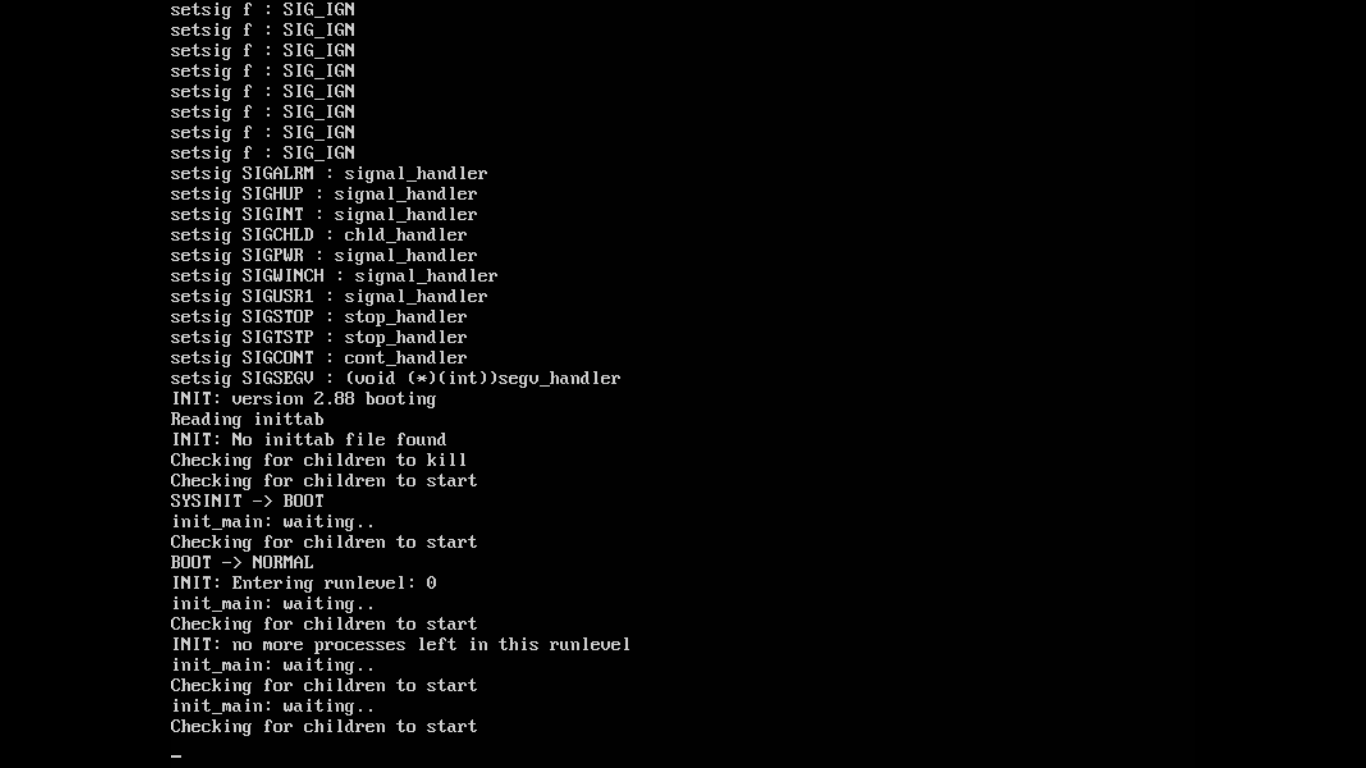
\includegraphics{./pictures/hack-daemon-init.png}
\caption{Daemon init 进程启动进入循环状态等待 request}
\end{figure}

此时,开启另外一个终端窗口,通过 cat request.dat \textgreater{}
/dev/.initctl 传送 request 请求包

{\begin{shaded}\begin{verbatim}
$ cat request.dat > /tmp/.initctl 
$ 
\end{verbatim}\end{shaded}}
观察 Daemon init 进程输出的调试信息,可以看到 init
进程已经识别出有一个修改 runlevel 的请求。

\begin{figure}[htbp]
\centering
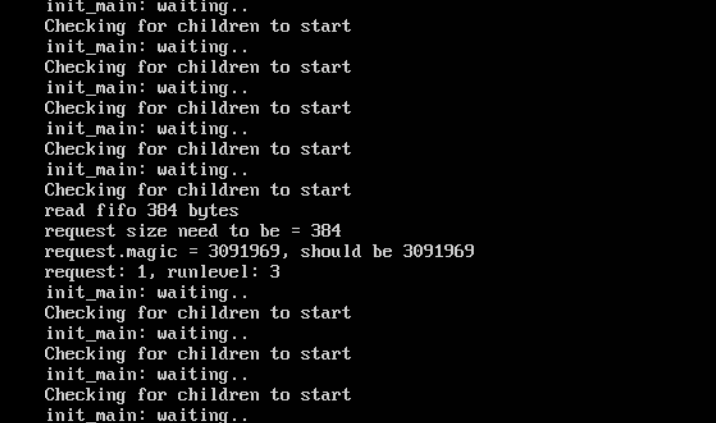
\includegraphics{./pictures/hack-init-fifo.png}
\caption{Daemon init 进程接到 init\_request 包}
\end{figure}

\section{案例2-umask掩码安全漏洞}

Linux内核的某些版本中,在umask设置为0000的情况下生成init进程。在这些版本的Linux,有些进程的初始化数据依赖于``init''的umask,并不自行设置。因为init进程生成系统重要而且敏感的文件,因而这种情况就可能形成漏洞问题。如果成功利用该漏洞,恶意用户就可以获取root权限,并破坏系统。

以下是可能会受到影响的 Linux 内核版本:

{\begin{shaded}\begin{verbatim}
Linux kernel 2.4.6
Linux kernel 2.4.5
+ Slackware Linux 8.0
Linux kernel 2.4.4
Linux kernel 2.4.3
\end{verbatim}\end{shaded}}
\subsection{umask用法简介}

umask和创建文件时的默认读写执行的权限相关,是和chmod命令密切相关的。

我们知道用 ls -l
命令查看文件权限,总共为4位(gid/uid,属主,组权,其它用户的权限),不过通常用到的是后3个。

例如,可以用chmod 755
file(此时这文件的权限是属主读(4)+写(2)+执行(1),同组的和其它用户有读写权限)

\subsection{umask的作用权限掩码}

默认情况下的umask值是022,可以用umask命令查看默认值。

此时,建立的文件默认权限是644,建立的目录的默认权限是755,因为建立文件的时候,默认本来就是没有可执行权限x的,而建立目录的时候,默认是可以执行的(也就是可以用
cd 进入)。

知道了umask的作用后,就可以修改umask的值了,例如:umask 024
则以后建立的文件和目录的默认权限就为642,753了

\subsection{参考资料}

\url{http://www.juniper.net/security/auto/vulnerabilities/vuln3031.html}

\url{http://user.ccidnet.com/tech/hack/2001/07/23/58_2766.html}

\section{案例3-利用脚本和符号链接攻击系统目录}

这个安全漏洞描述,是在 Debian 社区邮件列表中提出的。参考信息 BUGTRAQ ID:
52198

\url{http://bugs.debian.org/cgi-bin/bugreport.cgi?bug=661627}

因为这个漏洞是在于 init 执行脚本 x11-common
时,创建了一个临时目录,然后将临时目录的权限改为1777。这里,因为 init
脚本的执行是内核启动,以 root 权限执行的,所以执行脚本中的命令行时,也是
root 权限,就可能会造成安全漏洞。

\subsection{举例}

例如,如果用户提前根据创建一个符号链接文件,名字和 \$SOCKET\_DIR
相同,由于是符号链接,因此 33行的 if 语句不能成立,而36行通过 mkdir -p
操作因为之前 \$SOCKET\_DIR
存在,也不会覆盖原来的那个软链接文件。这样最初的软链接文件就获得了 root
权限,并且是 777 的可读可写可执行。一旦这个目录是系统 /etc/
目录,则可能就会导致用户有权限建立和删除文件,从而替换之前的系统文件,造成安全漏洞。

{\begin{shaded}\begin{verbatim}
    33    if [ -e $SOCKET_DIR ] && [ ! -d $SOCKET_DIR ]; then
    34      mv $SOCKET_DIR $SOCKET_DIR.$$
    35    fi
    36    mkdir -p $SOCKET_DIR
    37    chown root:root $SOCKET_DIR
    38    chmod 1777 $SOCKET_DIR
    [...]
    47    if [ -e $ICE_DIR ] && [ ! -d $ICE_DIR ]; then
    48      mv $ICE_DIR $ICE_DIR.$$
    49    fi
    50    mkdir -p $ICE_DIR
    51    chown root:root $ICE_DIR
    52    chmod 1777 $ICE_DIR
\end{verbatim}\end{shaded}}
这个漏洞产生的原因是,由于init脚本``x11-common''不安全方式创建``/tmp/.X11-unix''和``/tmp/.ICE-unix'',攻击者可以通过符号链接进行攻击,可能获得root特权。

\subsection{参考资料}

\url{http://www.jiangmin.com/zixun/3/2012-05-18/537.html}

\section{案例4-Android root 提权漏洞}

这篇文章中所提到的安全漏洞,也是和 init
进程有一定关系,但是并不在我们分析的 sysvinit
软件包中,也无法进行验证,仅供参考。

这个安全漏洞中,提到了一个 uevent 数据结构,是在 Linux 2.6
内核中设备驱动程序模型的一个重大调整。uevent事件(以前叫hotplug事件)
被用户出发后,会向内核传递消息,内核收到消息后,会进行解析和处理。

\subsection{举例}

文中提到了这样一条消息

{\begin{shaded}\begin{verbatim}
ACTION=addDEVPATH=/../data/local/tmpSUBSYSTEM=firmwareFIRMWARE=../../../data/local/tmp/hotplug
\end{verbatim}\end{shaded}}
通过函数parse\_event进行解析后,uevent的结构为:

{\begin{shaded}\begin{verbatim}
action="add"
path="/../data/local/tmp"
subsystem="firmware"
firmware="../../../data/local/tmp/hotplug"
\end{verbatim}\end{shaded}}
最后在内核load\_firmware函数,把hotplug中的数据写到
/proc/sys/kernel/hotplug 中,其内容变为
/data/local/tmp/exploid。这样就完成了让内核自动加载恶意程序,只要再次受到如wifi打开、usb插入等热拔插信息,内核就会以root权限加载恶意程序执行,从而达到提权的目的。

\subsection{参考资料}

结合init源码剖析android root提权漏洞

\url{http://hi.baidu.com/androidhacker/item/1954f41e301c0e773f87ceb0}

\chapter{Sysvinit 项目运行时调试图}

\section{Linux 内核启动 init 进程}

\subsection{start\_kernel}

{\begin{shaded}\begin{verbatim}
545 asmlinkage void __init start_kernel(void)
546 {
547         char * command_line;
548         unsigned long mempages;
549         extern char saved_command_line[];
550 /*
551  * Interrupts are still disabled. Do necessary setups, then
552  * enable them
553  */
554         lock_kernel();
555         printk(linux_banner);
556         setup_arch(&command_line);
557         printk("Kernel command line: %s\n", saved_command_line);
558         parse_options(command_line);
559         trap_init();
560         init_IRQ();
561         sched_init();
562         softirq_init();
563         time_init();
564 
.....
622         /* 
623          *      We count on the initial thread going ok 
624          *      Like idlers init is an unlocked kernel thread, which will
625          *      make syscalls (and thus be locked).
626          */
627         smp_init();
628         rest_init();
629 }
630 
\end{verbatim}\end{shaded}}
\begin{figure}[htbp]
\centering
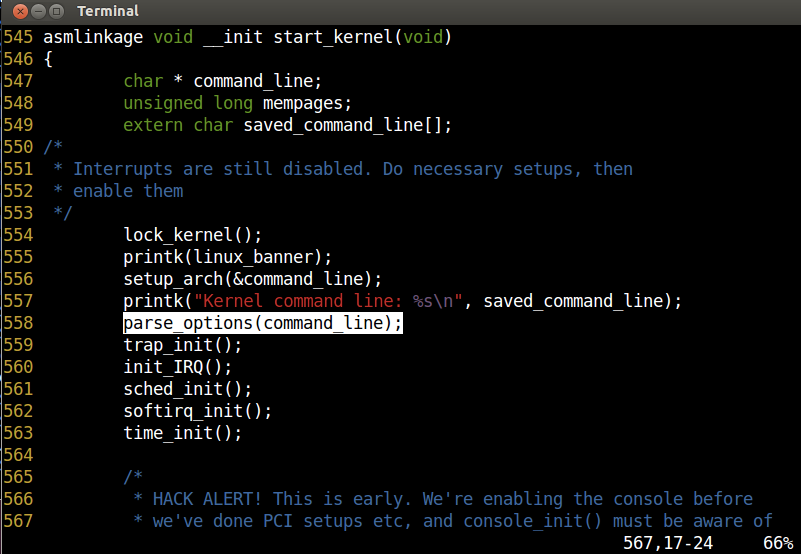
\includegraphics{./pictures/start_kernel.png}
\caption{内核start\_kernel函数}
\end{figure}

\subsection{parse\_options}

{\begin{shaded}\begin{verbatim}
426 static void __init parse_options(char *line)
427 {
428         char *next,*quote;
429         int args, envs;
430 
431         if (!*line)
432                 return;
433         args = 0;
434         envs = 1;       /* TERM is set to 'linux' by default */
435         next = line;
436         while ((line = next) != NULL) {
437                 quote = strchr(line,'"');
438                 next = strchr(line, ' ');
439                 while (next != NULL && quote != NULL && quote < next) {
440                         /* we found a left quote before the next blank
441                          * now we have to find the matching right quote
442                          */
443                         next = strchr(quote+1, '"');
444                         if (next != NULL) {
445                                 quote = strchr(next+1, '"');
446                                 next = strchr(next+1, ' ');
447                         }
448                 }
449                 if (next != NULL)
450                         *next++ = 0;
451                 if (!strncmp(line,"init=",5)) {
452                         line += 5;
453                         execute_command = line;
454                         /* In case LILO is going to boot us with default com      
\end{verbatim}\end{shaded}}
\begin{figure}[htbp]
\centering
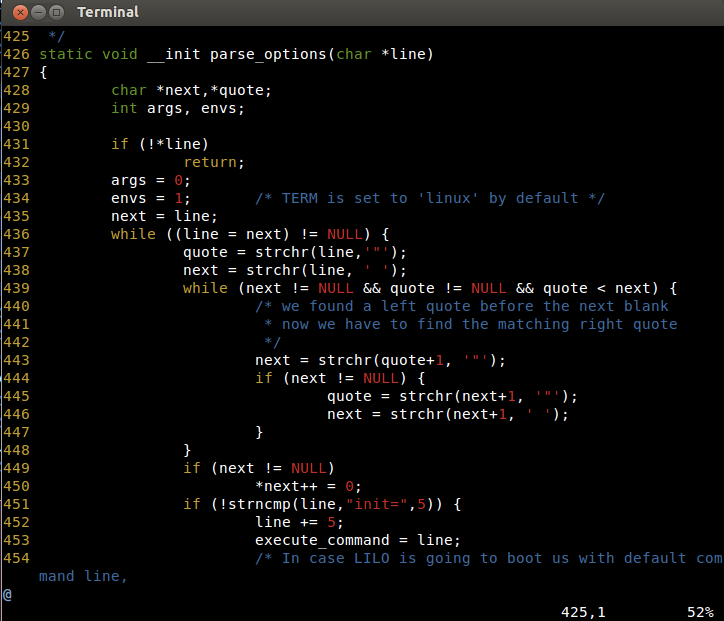
\includegraphics{./pictures/parse_options.png}
\caption{内核parse\_options函数}
\end{figure}

\subsection{rest\_init}

{\begin{shaded}\begin{verbatim}
532 
533 static void rest_init(void)
534 {
535         kernel_thread(init, NULL, CLONE_FS | CLONE_FILES | CLONE_SIGNAL);
536         unlock_kernel();
537         current->need_resched = 1;
538         cpu_idle();
539 }
540 
\end{verbatim}\end{shaded}}
\subsection{init 函数}

{\begin{shaded}\begin{verbatim}
805 static int init(void * unused)
806 {
807         lock_kernel();
808         do_basic_setup();
809 
810         prepare_namespace();
811 
812         /*
813          * Ok, we have completed the initial bootup, and
814          * we're essentially up and running. Get rid of the
815          * initmem segments and start the user-mode stuff..
816          */
817         free_initmem();
818         unlock_kernel();
819 
820         if (open("/dev/console", O_RDWR, 0) < 0)
821                 printk("Warning: unable to open an initial console.\n");
822 
823         (void) dup(0);
824         (void) dup(0);
825 
826         /*
827          * We try each of these until one succeeds.
828          *
829          * The Bourne shell can be used instead of init if we are 
830          * trying to recover a really broken machine.
831          */
832 
833         if (execute_command)
834                 execve(execute_command,argv_init,envp_init);
835         execve("/sbin/init",argv_init,envp_init);
836         execve("/etc/init",argv_init,envp_init);
837         execve("/bin/init",argv_init,envp_init);
838         execve("/bin/sh",argv_init,envp_init);
839         panic("No init found.  Try passing init= option to kernel.");
840 }
\end{verbatim}\end{shaded}}
\begin{figure}[htbp]
\centering
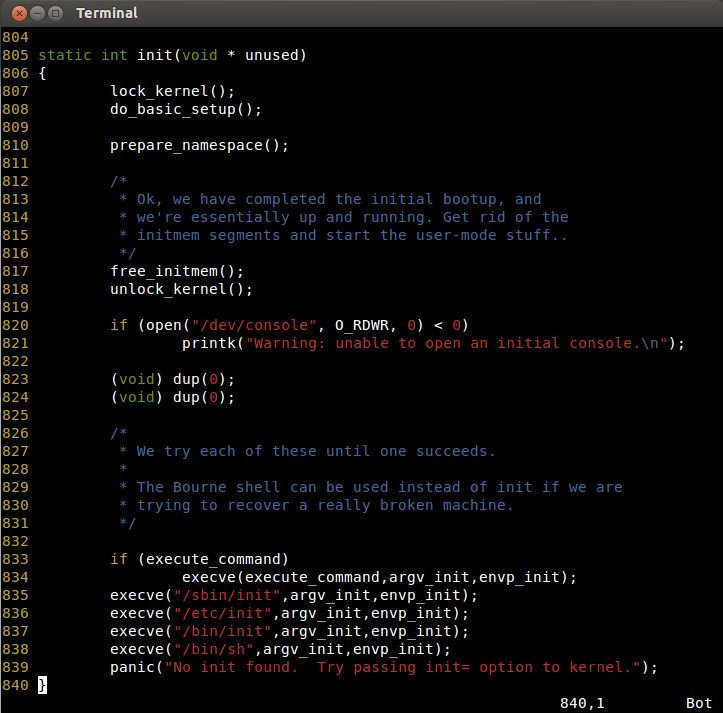
\includegraphics{./pictures/init.png}
\caption{内核init函数}
\end{figure}

至此我们找到了一条路径,使得内核从 start\_kernel 的主函数,进入到 init
进程。这里涉及到了4个重要的函数和1个重要的变量,这些都是和 init
进程如何启动直接相关的,对于我们了解在 init
进程启动之前的逻辑流程有重要作用。

\begin{itemize}
\item
  start\_kernel()
\item
  parse\_options()
\item
  rest\_init()
\item
  init()
\item
  execute\_command
\end{itemize}
我们用下面这张图来表示这些函数和变量之间的关系,可以更直观的看到内核启动init进程的流程。

\begin{figure}[htbp]
\centering
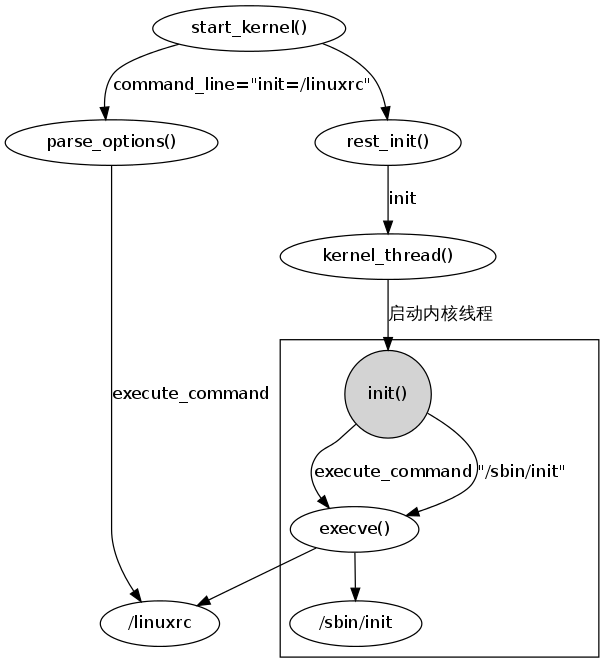
\includegraphics{./figures/kernel2init.png}
\caption{Linux 内核启动 init 进程}
\end{figure}

\section{init 进程和 telinit 之间的运行调试图}

\subsection{修改 INIT\_FIFO 改变两者联系的管道}

修改 initreq.h 头文件 33行处,定义为 /tmp/.initctl 以防和现在系统运行的
init 进程有关联

{\begin{shaded}\begin{verbatim}
$ vi initreq.h +33

 28 #if defined(__FreeBSD_kernel__)
 29 #  define INIT_FIFO  "/etc/.initctl"
 30 #else
 31 #  define INIT_FIFO  "/dev/initctl"
 32 #endif
 33 /* add by limingth */
 34 #undef INIT_FIFO
 35 #define INIT_FIFO  "/tmp/.initctl"
\end{verbatim}\end{shaded}}
\subsection{修改 Makefile ,加上 -DDEBUG 选项}

修改 Makefile 13行处,增加一个 -DDEBUG 11 CPPFLAGS = 12 CFLAGS ?= -ansi
-O2 -fomit-frame-pointer 13 override CFLAGS += -W -Wall -D\_GNU\_SOURCE
-DDEBUG 14 STATIC =

查看 init.h 头文件 64行处,INITDBG 通过 initlog 函数输出,无需修改

{\begin{shaded}\begin{verbatim}
 59 #if DEBUG
 60 #  define INITDBG(level, fmt, args...) initlog(level, fmt, ##args)
 61 #else
 62 #  define INITDBG(level, fmt, args...)
 63 #endif
\end{verbatim}\end{shaded}}
\subsection{修改 reboot 操作为打印语句,以防系统重启}

修改 reboot.h 头文件 50行处,将 init\_reboot 宏,修改为打印语句

{\begin{shaded}\begin{verbatim}
 50 #define init_reboot(magic)      reboot(magic)
 51 /* add by limingth */
 52 #undef init_reboot(magic)
 53 #define init_reboot(magic)      INITDBG(L_VB, "init_reboot: %d\n", magic)
 54 
\end{verbatim}\end{shaded}}
\subsection{修改源码中信号处理函数,以便直接中断 init 执行}

修改 init.c 源文件 102行处,注释掉注册信号处理函数的代码部分

{\begin{shaded}\begin{verbatim}
  93 /* Set a signal handler. */
  94 #define SETSIG(sa, sig, fun, flags) \
  95                 do { \
  96                         sa.sa_handler = fun; \
  97                         sa.sa_flags = flags; \
  98                         sigemptyset(&sa.sa_mask); \
  99                         sigaction(sig, &sa, NULL); \
 100                 } while(0)
 101 
 102 /* add by limingth */
 103 #undef SETSIG(sa, sig, fun, flags)
 104 #define SETSIG(sa, sig, fun, flags)     INITDBG(L_VB, "setsig %s : %s\t", #sig, #fun)
\end{verbatim}\end{shaded}}
\subsection{修改源码中关闭标准输出的部分,可以显示出调试信息}

{\begin{shaded}\begin{verbatim}
1049 #if 0
1050                 close(0);
1051                 close(1);
1052                 close(2);
1053 #endif

2591 #if 0
2592         close(0);
2593         close(1);
2594         close(2);
2595 #endif
\end{verbatim}\end{shaded}}
\subsection{在 Daemon 程序中插入打印当前获得 request 的信息}

{\begin{shaded}\begin{verbatim}
2278         initlog(L_VB, "request: %d, runlevel: %c\n", request.cmd, request.r     unlevel);
2279         switch(request.cmd) {
2280                 case INIT_CMD_RUNLVL:
\end{verbatim}\end{shaded}}
\subsection{重新编译运行 sudo ./init -i}

{\begin{shaded}\begin{verbatim}
$ sudo ./init -i 0
[sudo] password for akaedu: 
init_reboot: 0
setsig f : SIG_IGN  
...
setsig f : SIG_IGN  
setsig SIGALRM : signal_handler 
setsig SIGHUP : signal_handler  
setsig SIGINT : signal_handler  
setsig SIGCHLD : chld_handler   
setsig SIGPWR : signal_handler  
setsig SIGWINCH : signal_handler    
setsig SIGUSR1 : signal_handler 
setsig SIGSTOP : stop_handler   
setsig SIGTSTP : stop_handler   
setsig SIGCONT : cont_handler   
setsig SIGSEGV : (void (*)(int))segv_handler    
Reading inittab
Checking for children to kill
Checking for children to start
SYSINIT -> BOOT
init_main: waiting..
Checking for children to start
BOOT -> NORMAL
init_main: waiting..
Checking for children to start
\end{verbatim}\end{shaded}}
此时 init 进入 Daemon 循环中

\begin{figure}[htbp]
\centering
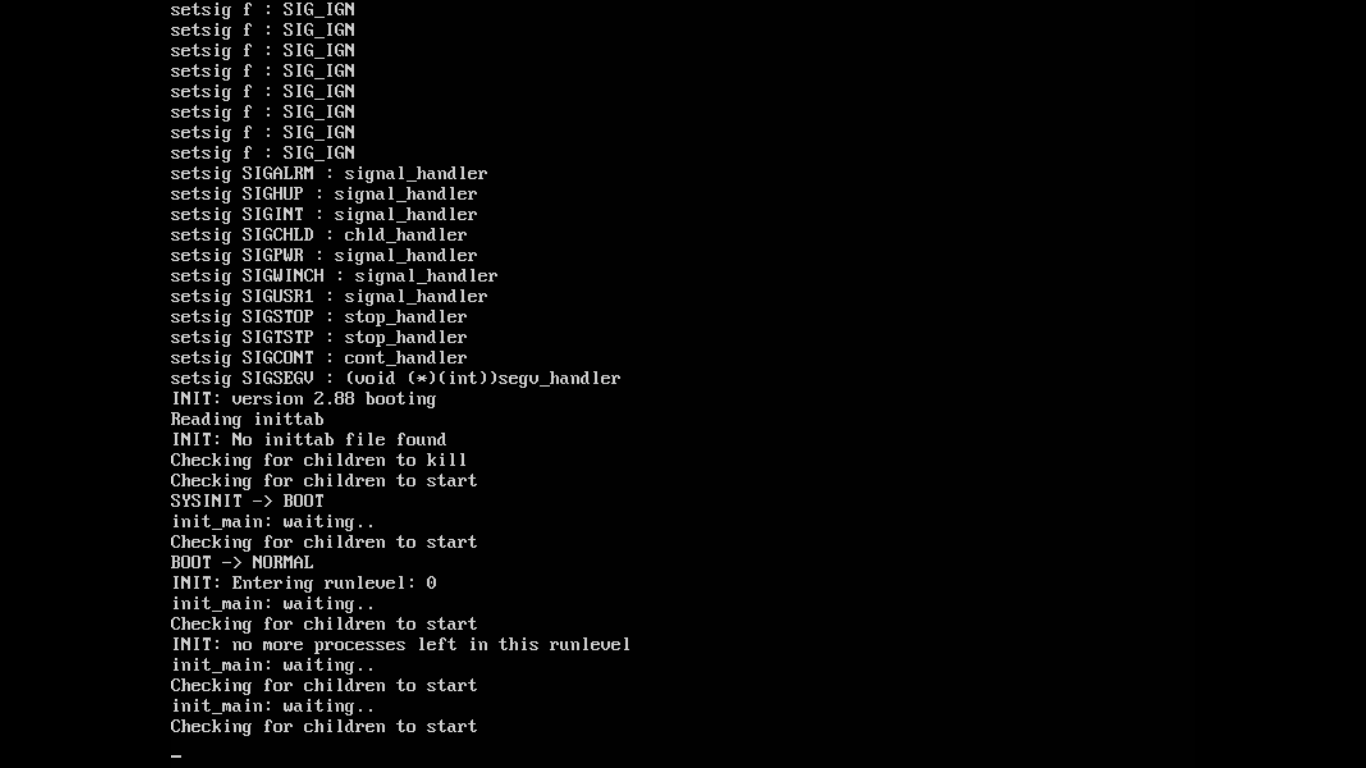
\includegraphics{./pictures/init-daemon-begin.png}
\caption{init 进入 Daemon 循环中}
\end{figure}

\subsection{启动 telinit 1 要求切换运行级别为单用户}

{\begin{shaded}\begin{verbatim}
$ sudo ./init 1
[sudo] password for akaedu: 
setsig SIGALRM : signal_handler 
write to INIT_FIFO
$ 
\end{verbatim}\end{shaded}}
我们运行了3次,分别要求改变运行级别为 1,5,7,这样就会通过 INIT\_FIFO
发送3次数据。

\begin{figure}[htbp]
\centering
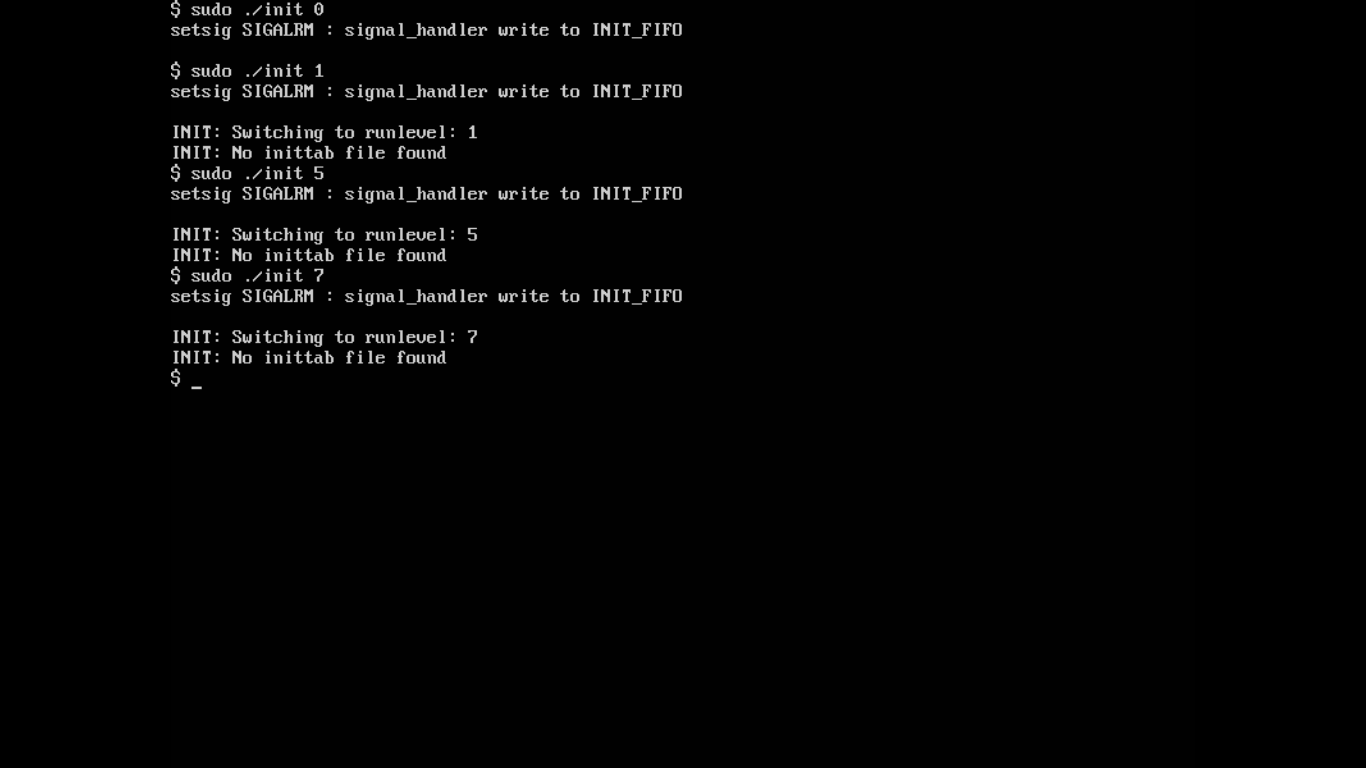
\includegraphics{./pictures/switch-to-runlevels.png}
\caption{init 更改运行级别的 request 请求}
\end{figure}

\subsection{查看 init 接收请求和处理方法}

可以看出通过 INIT\_FIFO ,init 方式2启动后,发送request请求,Deamon init
收到后可以打印出这个请求相关信息。

和请求级别相对应的,Daemon 也分别修改了3次级别,并仍然处于接收下一个
request 请求的循环中。

\begin{figure}[htbp]
\centering
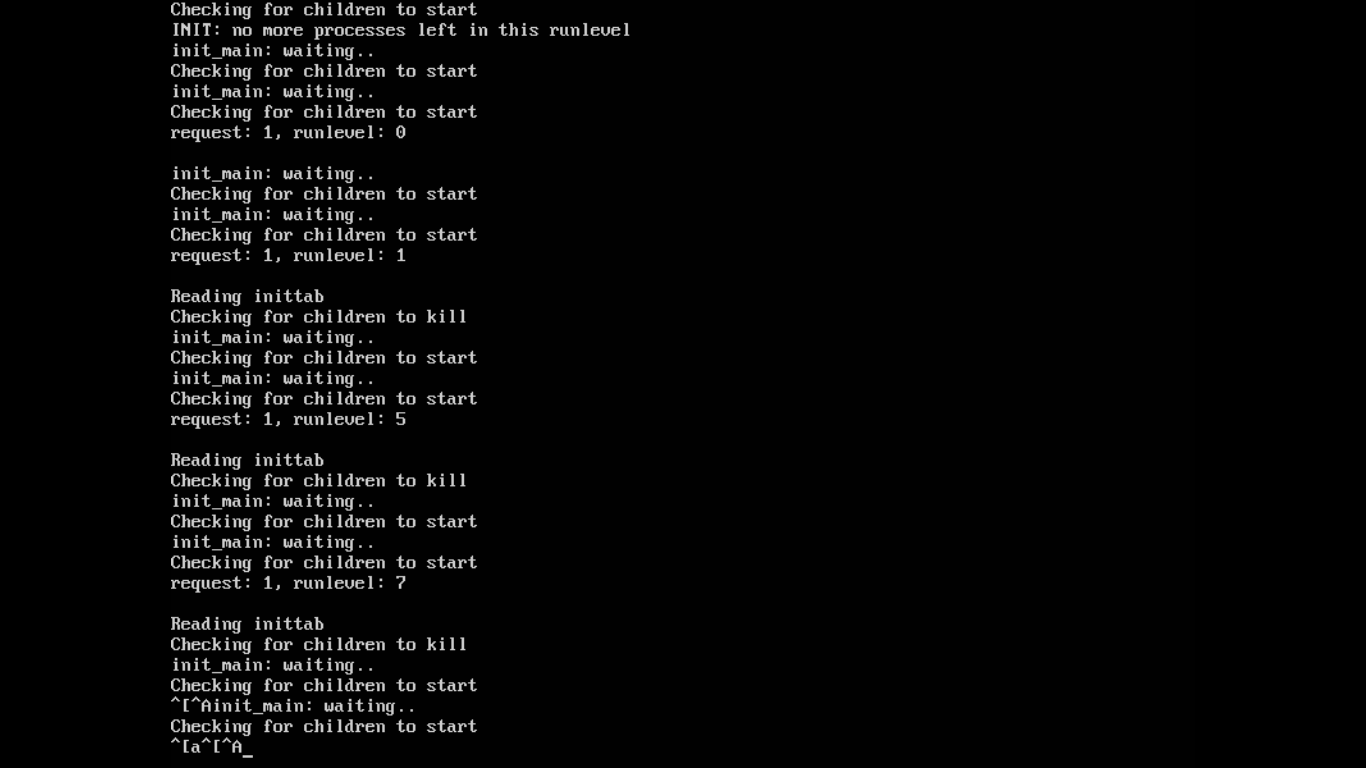
\includegraphics{./pictures/init-daemon-trans.png}
\caption{Daemon 收到运行级别的 request 请求}
\end{figure}

